\documentclass[times]{itmo-student-thesis}

%% Опции пакета:
%% - specification - если есть, генерируется задание, иначе не генерируется
%% - annotation - если есть, генерируется аннотация, иначе не генерируется
%% - times - делает все шрифтом Times New Roman, требует пакета pscyr.

%% Делает запятую в формулах более интеллектуальной, например:
%% $1,5x$ будет читаться как полтора икса, а не один запятая пять иксов.
%% Однако если написать $1, 5x$, то все будет как прежде.
\usepackage{icomma}

%% Данные пакеты необязательны к использованию в бакалаврских/магистерских
%% Они нужны для иллюстративных целей
%% Начало
% \usepackage{tikz}
% \usetikzlibrary{arrows}
% \usepackage{filecontents}
% \usepackage{wrapfig}

%% My packages
\usepackage{bbm}
\usepackage{graphicx}
\usepackage[
 font=small %% hack for bigger font size
 ]{subfig}
\usepackage{makecell}

%% Указываем файл с библиографией.
\addbibresource{thesis.bib}

\begin{document}

\studygroup{M3436}
\title{Анализ геномных перестроек с помощью случайных графов}
\author{Забелкин Алексей Андреевич}{Забелкина Алексея Андреевича}{Забелкин А.А.}{Забелкину А.А.}
\supervisor{Алексеев Никита Владимирович}{Алексеев Н.В.}{канд. физ.-мат. наук}{ведущий научный сотрудник Университета ИТМО}
\publishyear{2018}
%% Дата выдачи задания. Можно не указывать, тогда надо будет заполнить от руки.
\startdate{21}{ноября}{2017}
%% Срок сдачи студентом работы. Можно не указывать, тогда надо будет заполнить от руки.
%\finishdate{31}{мая}{2015}
%% Дата защиты. Можно не указывать, тогда надо будет заполнить от руки.
%\defencedate{15}{июня}{2015}

\secretary{Павлова О.Н.}


%% Эта команда генерирует титульный лист и аннотацию.
\maketitle{Бакалавр}

%% Оглавление
\tableofcontents

%% Макрос для введения. Совместим со старым стилевиком.
\startprefacepage

Для многих филогенетических исследований, изучающих эволюционные связи, является важной возможность оценивать эволюционное расстояние между различными видами.
Самое первое решение подобной задачи заключалось в оценке минимального расстояния, которое требуется для преобразования одного генома в другой.
Предположение о том, что для преобразования одного генома в другой было сделано минимальное число перестроек, называется предположением парсимонии.

Однако в реальном процессе эволюции данное предположение может не быть выполнено, поэтому необходимо иметь оценку, которая не будет опираться на предположение парсимонии.
Подобную оценку, которая оценивает реальное расстояние между двумя геномами, а не минимальное, принято называть истинным эволюционным расстоянием.
Данный термин впервые был предложен в \cite{termin}.

На данный момент уже существует несколько методов оценки эволюционнного расстояния.
В \cite{alexeev-1} показано, что истинное количество геномных перестроек между некоторыми видами дрожжей отличается от минимально возможного на $~20\%$, а также разработан метод для оценки этого истинного расстояния.
При этом в работе существенно использовали модель случайных графов Эрдеша-Реньи \cite{erdos}.
В статье \cite{fr-4} была высказана критика данной модели. В ней все геномные перестройки происходят равновероятно.
Но в реальной жизни некоторые регионы имеют больший шанс быть вовлеченными в перестройку, а некоторые меньшую.

В данной работе рассмотрена новая модель генома, предложенная в \cite{fr-4}.
Эта модель учитывает факт того, что разные регионы генома подвержены перестройкам в разной степени.
Также эта модель является <<хрупкой>> ~--- это означает, что только определенные <<хрупкие>> геномные области подвержены перестройкам.
Проведён эмпирический и теоретический анализ данной модели.
Построен алгоритм оценивания истинного эволюционного расстояния и проведено его сравнение с другими подходами.
\chapter{Обзор современных результатов в области сравнительной геномики и геномных перестроек}

\section{Виды геномных перестроек}

Геномные перестройки (англ. \textit{genome rearrangements}) ~--- это эволюционные события, которые меняют порядок генов на хромосомах.
Некоторые хромосомные области более подвержены перестройкам, чем другие.
Эта неустойчивость, как правило, обусловленая склонностью этих областей к смещению во время восстановления ДНК, усугубляется дефектами появления реплицирующих белков, которые повсеместно влияют на целостность генома.

\begin{figure}[h!]
    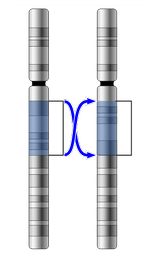
\includegraphics[width=1.5in]{img/reversal.png}
    \caption{Реверсия}
    \label{reversal}
\end{figure}

Самые распространенные геномными перестройками являются:
\begin{enumerate}
    \item Реверсия (инверсия) (англ. \textit{reversal}) ~--- разворот сегмента (рис.~\ref{reversal});
    \item Транслокация ~--- (анлг. \textit{translocation}) попарная замена сегментов двух хромосом;
    \item Слияние (англ. \textit{fusion}) ~--- объединение двух хромосом в одну;
    \item Расщепление (англ. \textit{fission}) ~--- разделение одной хромосомы на две.
\end{enumerate}

Все эти четыре типа перестановок могут быть смоделированы операцией Двойное-Разрезание-и-Склеивание (ДРС) (англ. \textit{Double-Cut-and-Join}) \cite{dcj}, которая <<разрезает>> хромосому в двух локациях и склеивает полученные регионы в другом порядке.

Также существуют более сложные геномные перестройки, которые могут быть смоделированы как разрез хромосом в $k$ локациях, где $k>2$, и склеивание полученных регионов в другом порядке.
Например, транспозиция (англ. \textit{transposition}).
В рамках данной работы эти перестройки рассматриваться не будут ввиду того, что происходят они достаточно редко, но при этом сильно усложняют получившуюся модель.
Рассмотрены будут все виды геномных перестроек, моделируемые с помощью ДРС, то есть $k=2$.

\section{Существующие методы оценки эволюционного расстояния}

\begin{figure}[h!]
    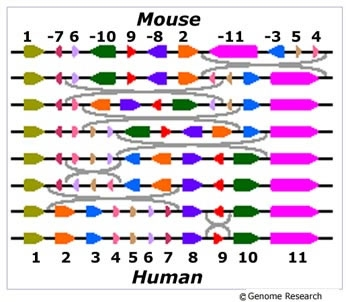
\includegraphics[width=4in]{img/mouse_human.jpg}
    \caption{Эволюционный сценарий}
    \label{mouse-human}
\end{figure}

Для любой оценки расстояния между двумя геномами мы предполагаем, что они имеют в себе одинаковый набор блоков, организованных в разном порядке.
Задача оценки расстояния сводится к задаче об оценке необходимого количества операций ДРС на соответствующих данным геномам графах.

\subsection{Оценка через минимальное расстояние}
Первым был предложен подход оценки расстояния как минимального необходимого, то есть минимального количества необходимых операций ДРС для перестройки одного генома в другой.
Появление данного подхода весьма закономерно и на данный момент используется в качестве нижней границы для оценки результатов.
Для геномов, которые слабо удалены друг от друга, данный метод даёт хорошие результаты.

Минимальное растоние определяется через <<граф точек разрыва>> (англ. \textit{breakpoint graph}.
Для восстановления эволюционного сценария решается задача сортировки.
Подобная задача сортировки с ипользованием только инверсий является NP-полной \cite{sorting-is-difficult}.

Но если рассматривать геномы, которые достаточно далеко удалены друг от друга, то ошибка даного алгоритма становится заметно выше.
Когда в реальности между генами могло произойти весьма большее количество перестроек, а природа их происхождения является случайной и не ведёт самым коротким путём, алгоритм оценки через минимальное расстояние будет же искать минимальный путь, который может отличаться от реального.

При большом количестве шагов ошибка данного метода в рамках модели, предложенной в данной работе, может достигать $50 \, \%$.
Но необходимо отметить, что с увеличением числа шагов происходит <<насыщение>> (англ. \textit{saturation}) модели, и любой алгоритм оценки расстояния начинает давать более плохие результаты.
В рамках построенной модели мы будем сравнивать получившийся алгоритм оценки с методом оценки через минимальное расстояние.

\subsection{Модель поломки случайных регионов}

В статье \cite{termin} был предложен метод для оценки истинного эволюционного расстояния, а также преложен сам термин <<истинного эволюционного расстояния>> (англ. \textit{true evolutionary distance}).
Однако, данный метод полагает, что геномы могут быть поломаны в любой позиции с равной вероятностью, то есть весь геном является <<хрупким>>.
Данное предположение, известное как модель поломок случайных регионов (ПСР-модель) (англ. \textit{random breakage model}) эволюции хромосом, было опровергнуто в пользу более строгой модели поломок хрупких регионов (ПХР-модели) (англ. \textit{fragile breakage model}) \cite{mouse}, в которой утверждается, что только определенные <<хрупкие>> (англ. \textit{fragile}) геномные области подвержены к перестановкам.
ПХР-модель поддерживается многими недавними исследованиями различных геномов (например, \cite{fragile}).
ПСР-модель можно рассматривать как экстремальный случай ПХР-модели, где каждая геномная область является хрупкой.

Таким образом, хотя в данной статье и был предложен алгоритм оценки, он не учитывает того факта, что некоторые регионы генома могут быть <<прочными>> (англ. \textit{solid}) и не имеют возможности сломаться. С точки зрения биологии это означает, что подобные изменения критичны и, скорее всего, ведут к гибели организма.

\subsection{Модель поломки хрупких регионов}
В статье \cite{alexeev-1} предложен новый метод оценки истинного эволюционного расстояния между двумя геномами в рамках ПХР-модели (модель поломки хрупких регионов).
Произведено оценивание предложенного метода для имитируемых геномов, которые показывают его высокую точность.

Для оценки истинного эволюционного расстояния в данной модели используется анализ так называемого <<графа точек разрыва>>.
Аналитически выведены формулы для распределения необходимых для оценки компонент и на основании этих формул преложен аналитический метод оценки истинного эволюционного расстояния.

Так как изучаемая нами модель является развитием и уточнением ПХР-модели, далее ПХР-модель будет рассмотрена подробнее.

\section{Анализ модели поломки хрупких регионов}
\subsection{Граф точек разрыва и двойной-разрез-и-склеивание}
Анализ начинается с круговых геномов и позже обращается к линейным геномам.
Геном с $n$ блоками представляется в виде графа генома, состоящего из $n$ направленных блоковых рёбер (англ. \textit{block edges}), кодирующих блоки и их границы, и $n$ неориентированных рёбер смежности (англ. \textit{adjacency edges}), кодирующих смежности между блоками.

\begin{figure}[h!]
    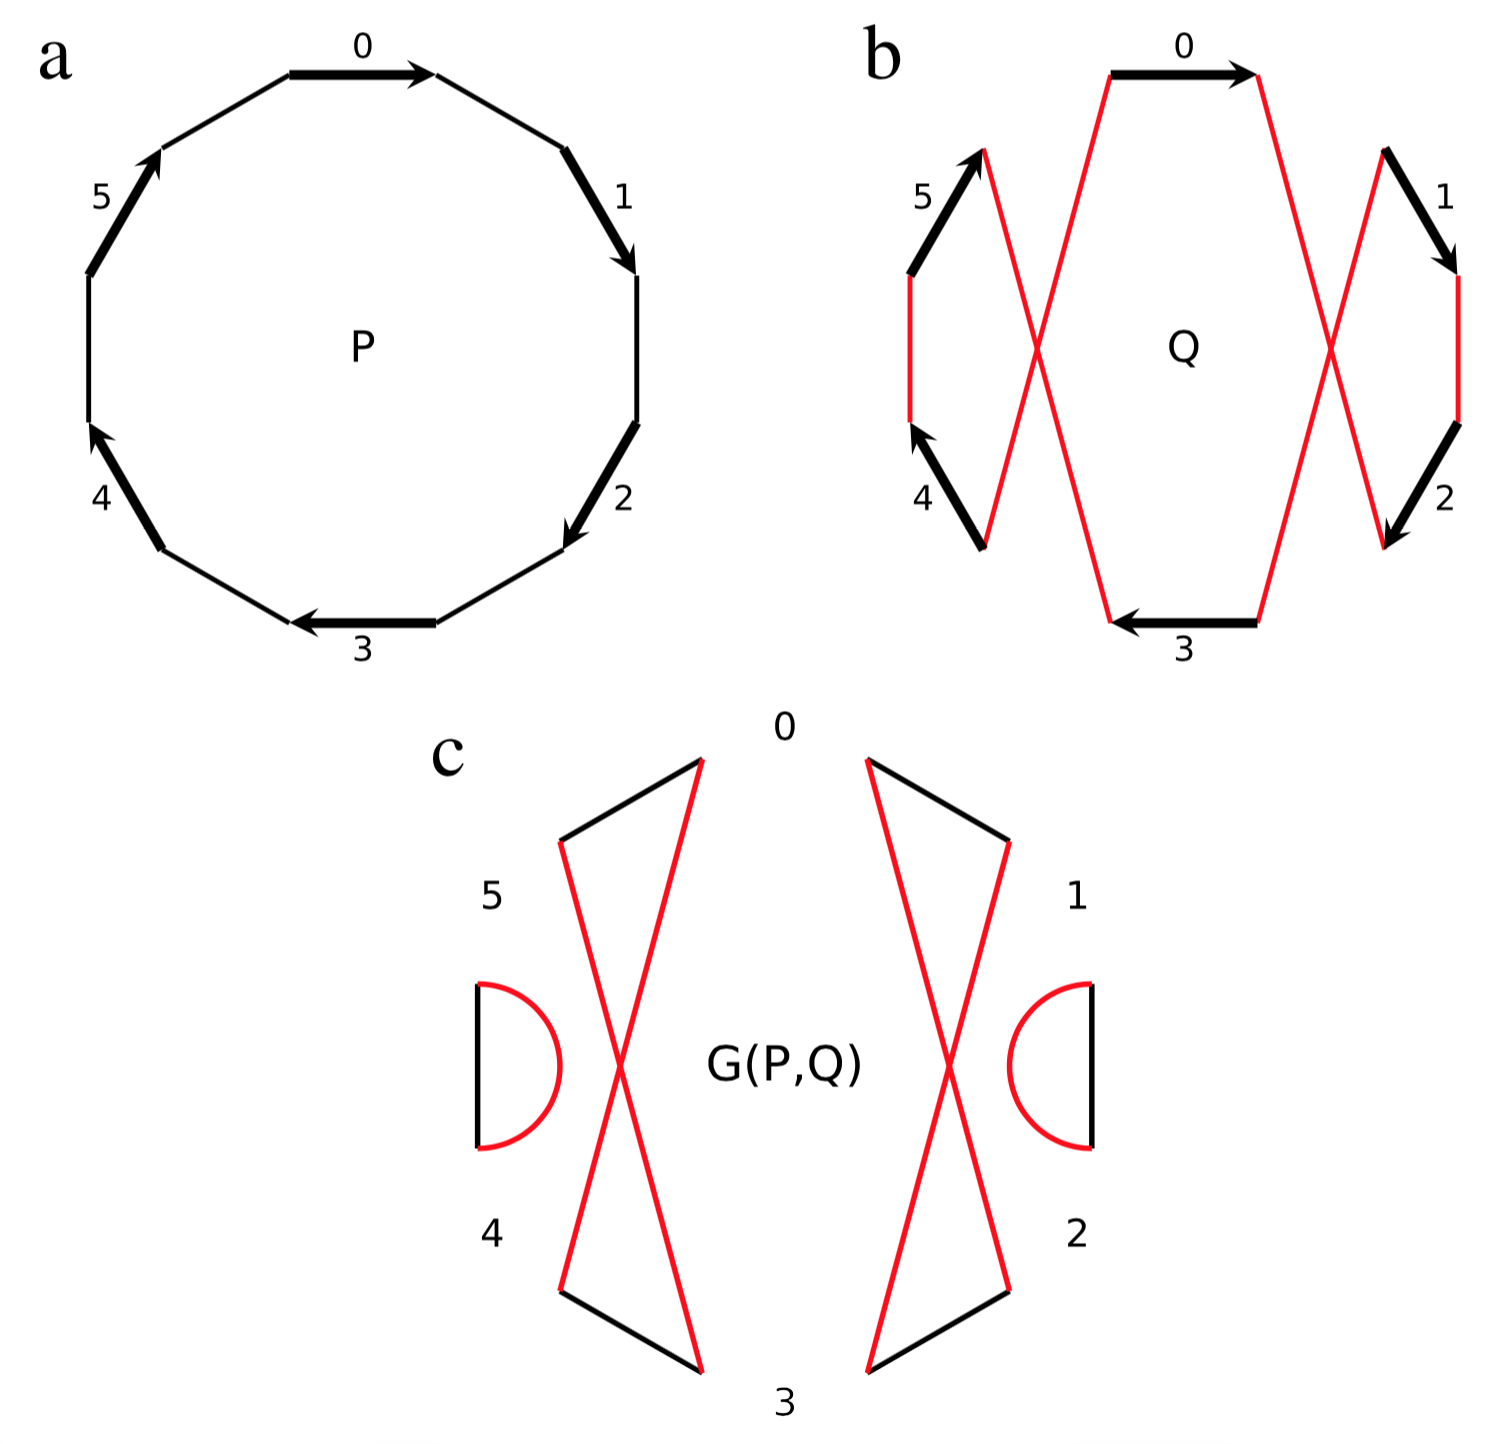
\includegraphics[width=4in]{img/genome_graph.png}
    \caption{
        \textbf{a} Геномный граф однохромосомного генома $P = (0, 1, 2, 3, 4, 5)$ с рёбрами смежности, окрашенными в черный цвет;
        \textbf{b} Геномный граф однохромосомного генома $Q = (0, -2, -1, 3, -5, -4)$ с рёбрами смежности, окрашенными в красный цвет;
        \textbf{c} Граф точек разрыва $G (P, Q)$ геномов $P$ и $Q$ представляет собой набор черно-красных циклов
        }
    \label{al-fig-1}
\end{figure}

Пусть $P$ и $Q$ --- геномы, содержащие один и тот же набор блоков.
Предположим, что в их графах геномов рёбра смежности $P$ окрашены в черный цвет (рис.~\ref{al-fig-1}a), а рёбра смежности $Q$ окрашены в красный цвет (рис.~\ref{al-fig-1}b).
Граф точек разрыва $G (P, Q)$ является суперпозицией графов генома $P$ и $Q$ с удаленными блоковыми рёбрами (рис.~\ref{al-fig-1}c).
Черные и красные рёбра смежности в $G (P, Q)$ образуют совокупность чередующихся черно-красных циклов.

Будем говорить, что черно-красный цикл является $l$-циклом, если он содержит $l$ черных ребер (и $l$ красных), а $c_l (P, Q)$ - число $l$-циклов в $G (P, Q)$. Важно отметить, что мы считаем рёбра только одного цвета, то есть на самом деле мы называем длиной половину числа ребер.
Циклы длины $1$ называют тривиальными, остальные нетривиальными.
Вершины нетривиальных циклов называются точками разрыва (англ. \textit{breakpoints}).

\begin{figure}[h!]
    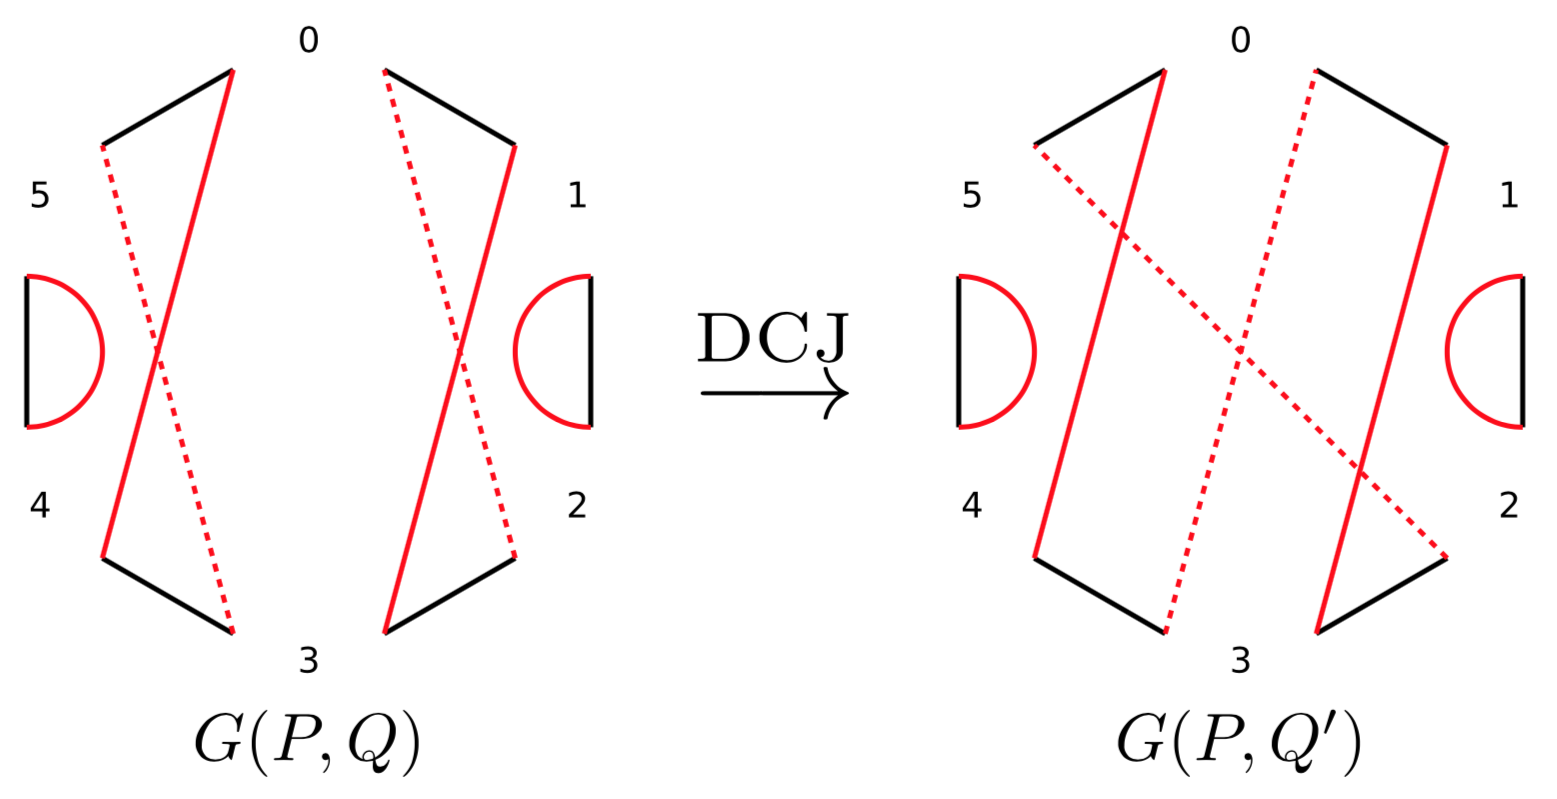
\includegraphics[width=5in]{img/dcj.png}
    \caption{операция ДРС в геноме $Q$ заменяет пару красных ребер в точке разреза $G (P, Q)$ другой парой красных ребер на тех же 4 вершинах}
    \label{al-fig-2}
\end{figure}

Операция ДРС в геноме $Q$ заменяет любую пару красных рёбер смежности $\{x, y\}, \{u, v\}$ другой парой ребер, состоящих из тех же вершин, то есть: $\{x, u\}, \{y, v\}$ либо $\{u, y\} , \{v, x\}$.
Говорится, что такая операция ДРС совершается на ребрах $\{x, y\}, \{u, v\}$ и их конечных точках (англ. \textit{endpoints}) $x, y, u, v$.
Операция ДРС в геноме $Q$, превращающая его в геном $Q'$, соответствует преобразованию графа точек разрава $G (P, Q)$ в граф точек разрыва $G (P, Q')$ (рис.~\ref{al-fig-2}).
Если ребра $\{x, y\}, \{u, v\}$ принадлежат разным циклам, то операция ДРС, осуществляемая на графе точек разрыва, объединяет два цикла в один, а если ребра $\{x, y\}, \{u, v\}$ принадлежат к одному и тому же циклу, то операция ДРС разбивает один цикл на два или сохраняет текущее количество циклов.
Минимальное количество операций ДРС, которое потребуется для преобразования $Q$ в $P$ назовём расстоянием ДРС (обозначается $d(P, Q)$) между геномами $P$ и $Q$.
Также введем ещё две компоненты: $b (P, Q) = \sum_{l \geq 2} l \cdot c_l(P, Q)$ --- половина общей длины всех нетривиальных циклов, $c (P, Q) = \sum_{l \geq 2} c_l(P, Q)$ --- количество циклов длины больше $1$.
Тогда для оценки на $d$ будет достаточно взять их разность: $d (P, Q) = b (P, Q) - c (P, Q)$.

\subsection{Эволюционная модель}
Задача эволюционной модели --- оценка истинного эволюционного расстояния между геномами $P$ и $Q$.
Будем считать, что геномы $P$ и $Q$ имеют один и тот же набор блоков, тогда в качестве процесса эволюции мы можем рассматривать дискретный марковский процесс.
Каждая операция ДРС в таком процессе происходит независимо, то есть у модели нет <<памяти>>, и с их помощью осуществляется последовательное превращение генома $P$ в геном $Q$.
Начальной точкой данного процесса является геном $Z = P$, конечной точкой является геном $Z = Q$.
Подобный процесс будет соответствовать преобразованию графа $G (P, P)$  в граф $G (P, Q)$.
Истинное эволюционное расстояние между $P$ и $Q$ будем оценивать как количество операций ДРС в данном преобразовании (число $k$).

Также важным замечанием является то, что даже при наличии тривиальных циклов в $G (P, Q)$, их количество является неизвестным параметром.
Это связано с тем, что мы не может точно сказать, является ли данный регион <<прочным>> или это <<хрупкий>> регион, который просто не был вовлечен в перестройку.
Для того, чтобы учитывать этот факт будем считать, что геномы $P$ и $Q$  составлены из большого числа $n$ прочных регионов ($n$ неизвестно), сменяющихся хрупкими регионами, причём некоторые регионы могли сохраниться случайно.
Подобные представления геномов $P$ и $Q$ обозначим $P_n$ и $Q_n$.
Далее будем рассматривать преобразование генома $P_n$ в геном $Q_n$ последовательностью операцией ДРС, которые происходят только на хрупких регионах.

Также важно, что, хотя число $n$ прочных областей неизвестно, графы точек разрыва $G (P, Q)$ и $G (P_n, Q_n)$ имеют одну и ту же структуру циклов, за исключением тривиальных циклов.
То есть, мы имеем $c_l (P_n, Q_n) = c_l (P, Q)$ для всех $l \geq 2$, что означает, в частности, $b (P_n, Q_n) = b (P, Q)$ и $c (P_n, Q_n) = c (P, Q)$, а следовательно $d (P_n, Q_n) = d (P, Q)$.
Графы точек разрыва $G (P, Q)$ и $G (P_n, Q_n)$ могут различаться только числом тривиальных циклов, а в нашей модели эта компонента считается неизвестной.

В рамках рассматриваемой эволюционной модели следующие параметры считаются известными, то есть наблюдаемыми:
\begin{enumerate}
    \item $c_l = c_l (P, Q)$ для $l \geq 2$ --- число циклов длины $l$ в $G (P, Q)$;
    \item $b = b (P, Q) = \sum_{l \geq 2} l \cdot c_l$ --- половина от общей длины всех циклов где $l \geq 2$ в $G (P, Q)$;
    \item $d = d (P, Q) = b - \sum_{l \geq 2} c_l(P, Q)$, --- минимальное необходимое количество операций ДРС (для преобразования $P$ в $Q$).
\end{enumerate}

Неизвестными, то есть ненаблюдаемыми, являются следующие параметры:
\begin{enumerate}
    \item $c_1 = c_1 (P_n , Q_n)$ --- число тривиальных циклов в $G(P_n , Q_n)$;
    \item $n$ --- половина общей длины всех циклов в $G(P_n , Q_n)$ или число хрупких регионов в геномах $P$ и $Q$;
    \item $k = k(P, Q)$ --- чило ДРС операций в Марковском процессе или истинное эволюционное расстояние между $P$ и $Q$.
\end{enumerate}

В качестве замечания необходимо отметить, что данная модель легко применяется к линейным геномам простым добавлением ребра между последним и первым блоками.

\subsection{Теоретический анализ и оценка расстояния}
В рамках данной модели основной задачей является оценка неизвестных параметров через известные.
Для всех необходимых компонент аналитически выведем необходимые формулы.

Количество циклов заданной длины можно посчитать по формуле:
$$c'_{n,k,m}=
\frac{\binom{k}{m-1}\binom{n-m}{2}^{k-m+1}m^{m-2}m!}
{\binom{n}{2}^k},$$
где $n$ --- число вершин, $k$ --- число шагов, $m$ --- длина цикла

Переходя к пределу, получим:
$$\frac{c_l} n = \frac {c'_{n,k,m}} n \xrightarrow[n \to \infty]{[k=\frac{n \gamma}{2}]} \frac{e^{-\gamma l} \gamma^{l-1} l^{l-2}} {l!},$$
где $\gamma = \frac {2k} n$ --- число произошедших перестроек, нормированное относительно общего числа областей

Далее оцениваются нормированные величины $d$ и $b$:

$$\frac b n = 1 - e ^ {- \gamma} + o(1)
\qquad
\frac d n = 1 - \sum_{l=1}^{\infty} \frac {p_l} l + o(1),$$
$$p_l = e^{-\gamma l} \frac {(\gamma l)^{l-1}}{l!}$$

После этого мы можем оценить величину $\frac d b$ отдельно от $n$:
$$\frac d b \approx  \frac {1 - \sum_{l=1}^{\infty} e^{-\gamma l} \frac {(\gamma l)^{l-1}}{l \cdot l!}}{1 - e ^ {- \gamma}} \, .$$

Но величины $d$ и $b$ известны в рамках данной модели, и мы знаем формулу зависимости $\gamma$ от этих величин.
А также известно, как величина $\frac b n$ зависит от $\gamma$.
Зная эти зависимости, получаем формулу для неизвестных нам $n$ и $k$:
$$n_e = \frac b {1 - e^{-\gamma_e}}
\qquad
k_e = \frac {\gamma_e \cdot n_e} {2},$$
\centerline{где $n_e$ --- оценка на количество хрупких регионов,}
\centerline{$k_e$ --- оценка на истинное эволюционное расстояние}

\begin{figure}[h!]
    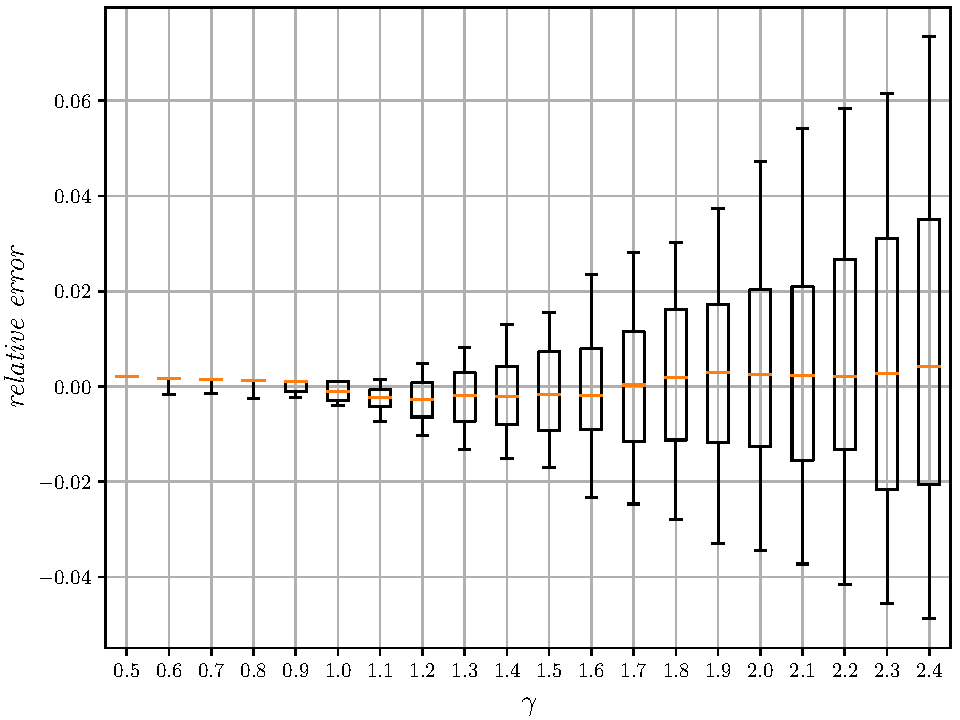
\includegraphics[width=.8\linewidth]{img/classic_est_error.pdf}
    \caption{Зависимость распределения относительной ошибки $\frac {k_e - k} k$ от $\gamma$ }
    \label{classic-est-error}
\end{figure}
Для оценки качества работы данного метода проведём 200 независимых экспериментов с моделируемым Марковским процессом построим график вида <<ящик с усами>> (рис.~\ref{classic-est-error}).

На данном графике и во всех подобных графиках далее <<ящикам>> соответствует $50 \, \%$ результатов, а усам $90 \, \%$.
Как мы видим, данный метод в $90 \, \%$ случаев ошибается не более, чем на $7 \, \%$, что является отличным показателем.
Но, к сожалению, данная модель имеет и недостатки, критика была высказана в \cite{fr-4}.

Дело в том, что выбор рёбер в Марковском процессе происходит равновероятно, в то время как в реальной жизни некоторые регионы имеют больший шанс быть вовлеченными в перестройку, а некоторые меньшую.
Данное замечание послужило мотивацией для создания модели, представленной  в данной работе.

\section{Описание модели Дирихле}

\subsection{Снабжения графа точек разрыва весами}
Аналогично ПХР-модели модель Дирихле использует граф точек разрыва для представления геномов.
В данной модели мы будем считать, что у каждого хрупкого региона есть некоторая вероятность быть вовлеченным в перестройку.

\begin{figure}[h!]
    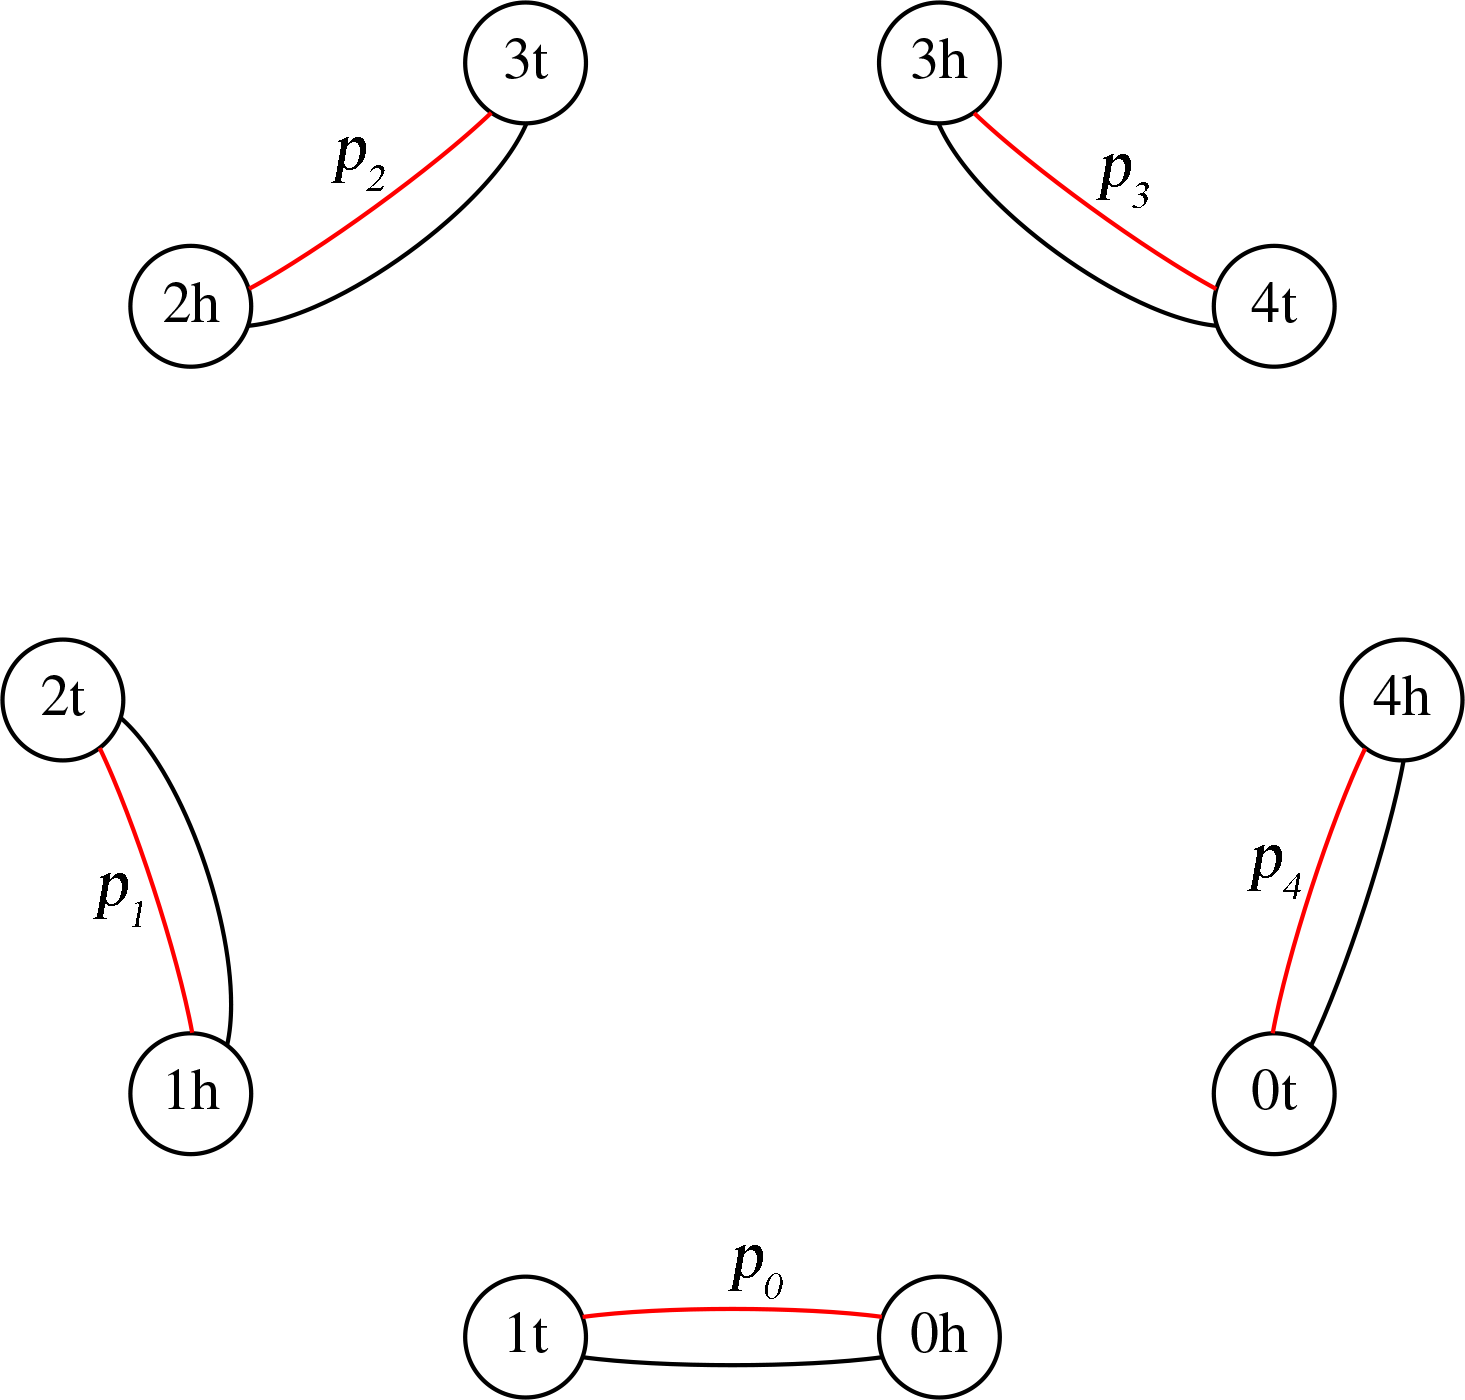
\includegraphics[width=4in]{img/bpg0-eps-converted-to.png}
    \caption{Граф точек разрыва с весами}
\end{figure}

Пусть $n$ --- это размер геномов $P$ и $Q$.
Каждое красное ребро в графе снабдим соответствующим числом $p_i$ --- его вероятностью быть вовлеченным в перестройку.
$\sum_{i=0}^{n-1} {p_i} = 1$ по определению.

\subsection{Модификация операции двойной-разрез-и-склеивание}
Операция ДРС также производится на красных ребрах.
Но теперь помимо рёбер смежности она принимает и вероятности, подписанные на этих ребрах.

Пусть операция ДРС производится на рёбрах с номерами $i$ и $j$ и соответствующие рёбра смежности --- это $\{x, y\}, \{u, v\}$, а вероятности --- $p_i$ и $p_j$.
Эта операция аналогично заменяет данные рёбра другой парой рёбер, образующих паросочетания на тех же вершинах, что и исходные, то есть $\{x, u\}, \{y, v\}$ либо $\{u, y\} , \{v, x\}$.
Также перераспределяются и веса.
Новые веса $p_i'$ и $p_j'$ будут равны $r_1 \cdot p_i + r_2 \cdot p_j$ и $(1 - r_1) \cdot p_i + (1 - r_2) \cdot p_j$ соответственно, где $r_1$ и $r_2$ --- случайные числа из отрезка $(0, 1)$.

\begin{figure}[h!]
    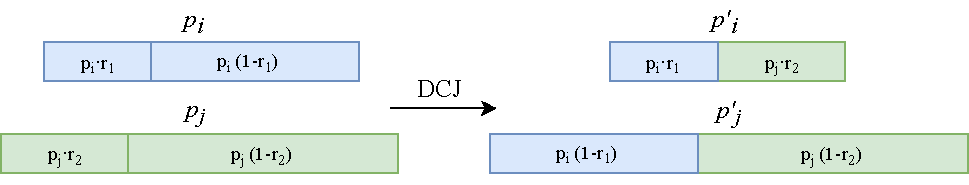
\includegraphics[width=\linewidth]{img/weights-redistribution.pdf}
    \caption{Пример перераспределения весов}
    \label{weights-redistribution}
\end{figure}

Указанное перераспределение весов предложено в статье \cite{fr-4}, и соответствующие веса и правила перераспределения весов обусловлены биологически.
В реальной жизни вероятность поломки какого-либо региона зависит от множества факторов.
Геном имеет достаточно сложную трёхмерную структуру \cite{3d} и вероятность поломки региона тесно связана с физическим устройством генома.
В данной работе мы придерживаемся мнения о том, что хрупкие регионы являются участками открытого хроматина.
В предположении, что хрупкие регионы являются участками открытого хроматина, хрупкий регион может сломаться в любом своём месте. Считается, что вероятность быть вовлеченным в перестройку пропорциональна длине этого региона.

Каждый регион, вовлеченный в перестройку, равновероятно ломается в случайном месте своей длины, что соответствует числам $r_1$ и $r_2$.
И далее веса перераспределяются в соответствии с местами этих поломок, сохраняя общую сумму вероятностей (для примера см. Рис.~\ref{weights-redistribution}).

\subsection{Эволюционная модель и равновесное распределение}
Как и в ПХР-модели, рассмотренной ранее, для оценки истинного эволюционного расстояния между геномами $P$ и $Q$, которые имеют один и тот же набор блоков, будем рассматривать процесс эволюции как дискретный Марковский процесс, который начинается с генома $P$ и заканчивается геномом $Q$.
Подобное преобразование, как и ранее, осуществляется с помощью последовательности операций ДРС.

Отличие заключается в том, что на каждом шаге Марковского процесса выбор ребра происходит не равновероятно, а соответствует вероятностям, написанным на соответствующих рёбрах.
То есть вероятность того, что $2$ ребра с номерами $i$ и $j$ будут вовлечены в перестройку, будет равна $p_i \cdot p_j$ (выбор происходит независимо).

Полученный марковский процесс является:
\begin{enumerate}
    \item Реверсивным, то есть время возвращения в некоторое состояние имеет конечное математическое ожидание;
    \item Непериодичным, так как существует ненулевая вероятность остаться в текущем состоянии;
    \item Неразложимым, то есть любое состояние процесса может быть достигнуто из любого другого состояния за конечное число шагов. Это свойство может быть проверено простым упорядочиванием состояний и математической индукцией. \\
\end{enumerate}
Следовательно, этот марковский процесс сходится \cite{teor-ver}.
Как показано в \cite{fr-4}, стационарное распределение этого процесса -- это равномерное распределение на всех векторах $p = \{p_i\}$, сумма которых равна $1$.
Это распределение является плоским распределением Дирихле.

Для того, чтобы получить данное распределение, достаточно выбрать отдельные вероятности как распределенные по экспоненциальному закону и нормализовать \cite{generation}:
$$\text{Пусть} \, i \in \{1, 2, \ldots, n\}, \qquad \alpha_i = Exp(1), \qquad M = \sum_{i=0}^n \alpha_i,$$
$$\text{тогда} \,\, (p_1, p_2, \ldots, p_n) 
= \left(\frac {\alpha_1} M, \frac {\alpha_2} M, \ldots, \frac {\alpha_n} M\right) 
= Dir(1, 1, \ldots, 1).$$

\chapterconclusion
В главе 1 были рассмотрены известные на данный момент методы для оценки эволюционного расстояния: оценка через минимальное расстояние, модель поломки случайных регионов, модель поломки хрупких регионов. Несмотря на то, что в рамках рассмотренных моделей можно получать достаточно точные результаты относительно истинного эволюционного расстояния, все они не учитывают некоторых биологических особенностей генома, например, факт того, что разные хрупкие регионы могут иметь разную вероятность быть вовлеченными в перестройку.

Была описана модель устройства генома, более точно учитывающая структуру ДНК (модель Дирихле). В дальнейшем будет проведён анализ именно этой модели.
\chapter{Анализ модели Дирихле}

\section{Математическое ожидание числа циклов заданной длины}
Одним из самых важных параметров модели является число циклов заданной длины.
Для простоты изложения сначала будут рассмотрены циклы с конкретными и малыми длинами ($1$ и $2$).
Далее эти рассуждения будут обобщены на циклы произвольной длины $m$.

\subsection{Подсчет циклов длины один}
Для начала оценим число циклов единичной длины.
То есть это либо те циклы, которые не были затронуты в марковском процессе, либо те, которые были получены из рапада цикла большой длины.

Здесь и далее будем считать, что циклы заданной длины образуются только в результате слияния циклов меньшей длины, так как второй сценарий намного менее вероятен.
Этот факт подтверждается сравнением аналитических и эмпирических результатов, которое будет приведено впоследствии.
И это сравнение позволяет оценить погрешность, которая получается в условиях такого предположения.
Это погрешность оказывается пренебрежимо малой.

Также считаем, что число хрупких регионов $n$ достаточно большое, и впоследствии переходим к пределу по $n$; в то же время, длины циклов $m$ полагаем фиксированными. Полагаем, что $k$ и $m$ имеют один порядок, а именно: $$\exists \, \gamma \sim \frac {2k} n : \gamma \neq 0 \, \textrm{и} \, \gamma \neq \infty \, .$$

Итак, зафиксируем ребро номером $i$, его вероятность быть вовлеченным в перестройку равна $p_i$.
Так как шагов всего $k$, и на каждом шаге выбирается $2$ ребра, вероятность, что $i$-ое ребро никогда не участвовало в перестройке равно $(1 - p_i) ^ {2k}$.

Вычисляя математическое ожидание (подразумеваем математическое ожидание по Марковскому процессу) считаем, что $p_i$ фиксированы. Для учёта вероятностей $p_i$ далее берется интеграл по плотности вероятности. В данном случае мы можем считать $p_i$ фиксированными для всего Марковского процесса, так как оперируем стационарным распределением.

\def \indicator {\mathbbm{1}}
Общее число циклов длины один $c_1$ равно $\sum_i \indicator_{\{i\textrm{-е ребро не участвовало в перестройках}\}}$.
Среднее нормированное число циклов длины $1$ равно:

$$E \left( \frac {c_1} n \right) = \frac 1 n \sum_i (1 - p_i)^{2k} \, .$$
Далее перейдём к пределу по $n$, а $p_i$ распишем как нормированные экспоненциальные величины $\alpha_i$, где $M = \sum_i \alpha_i$:

Заметим, что если $a$ конечно, то по центральной предельной теореме выполняется:
$$
    \left(\frac M n \right)^a =
    \left(\frac {n + \xi \sqrt{n}} n \right)^a =
    \left(1 + \frac \xi {\sqrt{n}} \right)^a
    \xrightarrow[n \to \infty]{} 1 \, .\label{clt}
$$

По доказанному утверждению $\frac {2k} M \xrightarrow[n \to \infty]{} \gamma$, тогда
$$
	E \left( \frac {c_1} n \right) =
    \frac 1 n \sum_i (1 - \frac {\alpha_i} M)^{2k}
    \xrightarrow[n \to \infty]{[k=\frac{n \gamma}{2}]}
    \frac 1 n \sum_i e^{- \gamma \alpha_i}
    (1 + o(1)) \, .
$$

Проинтегрируем по плотности вероятности:
$$
\frac 1 n \sum_i \intop_{0}^{\infty} e^{- \gamma \alpha_i} e^{-\alpha_i} {\mathrm{d} \alpha_i}
\sim \frac 1 n \sum_i \intop_{0}^{\infty} e^{- \alpha_i (\gamma + 1)} {\mathrm{d} \alpha_i}
\sim \frac 1 n \sum_i \frac 1 {1 + \gamma}
\sim \frac 1 {1 + \gamma} \, .
$$

\subsection{Подсчет циклов длины два}
Для того, чтобы посчитать число циклов длины 2, зафиксируем два ребра $i$ и $j$, образовавшие этот цикл.
Всего шагов произошло $k$, и на каком-то из этих шагов эти два ребра были вовлечены в перестройку, следовательно, необходимо домножить на $k$.
На протяжении всех остальных шагов эти рёбра затронуты не были, значит необходимо так же домножить на $(1 - p_i - p_j) ^ {2 (k - 1)}$.
Получаем формулы для вероятности $k \cdot p_i \cdot p_j (1 - p_i - p_j) ^ {2 (k - 1)}$.
Далее суммирием эти вероятности по всем возможным $i$ и $j$.
Среднее нормированное число циклов длины $2$ равно:
$$E \left( \frac {c_2} n \right) =
\frac 1 n \sum_i \sum_j
k p_i p_j (1 - p_i - p_j) ^ {2 (k - 1)} \, .$$

Аналогично распишем $p_i$ через $\alpha_i$:
$$E \left( \frac {c_2} n \right) =
\frac 1 n \sum_i \sum_j
k \frac{\alpha_i \alpha_j} {M^2} (1 - \frac{\alpha_i + \alpha_j} M) ^ {2 (k - 1)} = $$
$$ = \frac k {n M^2} \sum_i \sum_j
\alpha_i \alpha_j (1 - \frac{\alpha_i + \alpha_j} M) ^ {2 (k - 1)}
\sim
\frac \gamma {2 M^2} \sum_i \sum_j
\alpha_i \alpha_j e^{- \gamma \alpha_i} e^{- \gamma \alpha_j}
(1 + o(1)) \, .$$

Проинтегрируем по плотности вероятности:
$$
\frac \gamma {2 M^2} \sum_i \sum_j
\intop_{0}^{\infty} \intop_{0}^{\infty}
\alpha_i \alpha_j e^{- \gamma \alpha_i} e^{- \gamma \alpha_j} e^{- \alpha_i} e^{- \alpha_j}
{\mathrm{d} \alpha_i} {\mathrm{d} \alpha_j} \sim 
$$ $$
\sim \frac \gamma {2 M^2} \sum_i \sum_j
\intop_{0}^{\infty} \intop_{0}^{\infty}
\alpha_i \alpha_j e^{- \alpha_i (\gamma + 1)} e^{- \alpha_j (\gamma + 1)}
{\mathrm{d} \alpha_i} {\mathrm{d} \alpha_j}
\sim \frac \gamma {2 M^2} \sum_i \sum_j
\frac 1 {(1 + \gamma)^4} \sim 
$$ $$
\sim \frac {n^2 \gamma} {2 M^2 (1 + \gamma)^4} \sim \frac {\gamma} {2 (1 + \gamma)^4} \, .
$$

\subsection{Основная теорема}
\begin{theorem}
Пусть геном $P_n$ --- геном с $n$ хрупкими регионами и геном $Q_n$ получен из $P_n$ посредством $k = \frac {\gamma n} 2$ операций ДРС для $\gamma > 0$.

Тогда для любого фиксированного $m$ среднее нормированное число циклов длины $m$ в $G(P_n, Q_n)$ равно:
$$	E \left( \frac {c_m} n \right)
	\xrightarrow[n \to \infty]{}
	\frac
    {(3 m - 3)! \gamma^{m-1}}
    {m! (2 m - 1)! (\gamma + 1) ^ {3 m - 2}} \, .
$$
\end{theorem}
\begin{proof}

Для простоты прочные фрагменты будем называть блоками.
Для начала необходимо выбрать блоки, из которых будет получен цикл, всего блоков $n$, нам необходимо $m$, зафиксируем необходимые блоки домножив на $\binom{n}{m}$.
Для образования цикла длины $m$ нужно произвести $m - 1$ шаг, всего шагов $k$, зафиксируем необходимые шаги домножив на $\binom{k}{m-1}$.

Далее, когда зафиксированы блоки и шаги, на которых они будут сливаться,  нужно получить сумму вероятностей по всем возможным сценариям их слияния в цикл длины $m$.
По лемме ~\ref{l-prufer} эта вероятность равна
$2 ^ {m - 1} (m - 1)! p_1 \ldots p_m (p_1 + \ldots + p_m) ^ {m - 2}$.
И на всех остальных $k - m + 1$ шагах необходимо не затрагивать выбранные $m$ рёбер, это записывается как $(1 - \sum_{i=1}^{m} p_i) ^ {2 (k - m + 1)}$.

$$	E \left( \frac {c_m} n \right) =
    \frac 1 n
    \binom{n}{m}
    \binom{k}{m-1}
    2 ^ {m - 1} (m - 1)! p_1 \ldots p_m (p_1 + \ldots + p_m) ^ {m - 2}
    \times
    $$ $$
    \times
    (1 - \sum_{i=1}^{m} p_i) ^ {2 (k - m + 1)} \, .%точка
$$
 
Распишем $p_i$ через $\alpha_i$ и раскроем биномиальные коэффициенты: 
$$  E \left( \frac {c_m} n \right) \sim
	\frac 1 n
    \cdot \frac {n^m} {m!}
    \cdot \frac {k^{m-1}} {(m-1)!}
    2 ^ {m - 1} (m - 1)! \frac {\alpha_1} M \ldots \frac {\alpha_m} M 
    \left(\frac {\alpha_1} M + \ldots + \frac {\alpha_m} M\right) ^ {m - 2}
    \times
    $$ $$
    \times
    (1 - \sum_{i=1}^{m} \frac {\alpha_i} M) ^ {2 (k - m + 1)}
    \sim
$$

$$  \sim
	\frac {n^{m-1} k^{m-1} } {m!}
    \cdot \frac {2 ^ {m - 1}} {M^{2m-2}}
    \alpha_1 \ldots \alpha_m
    (\alpha_1 + \ldots + \alpha_m) ^ {m - 2}
    e ^ {- \sum_{i=1}^{m} \alpha_i}
    \sim
$$
$$  \sim
	\frac 1 {m!}
	\left(\frac {2 k} {M} \right)^{m-1}
    \left(\frac n M\right)^{m-1}
    \alpha_1 \ldots \alpha_m
    (\alpha_1 + \ldots + \alpha_m) ^ {m - 2}
    e ^ {- \sum_{i=1}^{m} \alpha_i}
    \sim
$$
$$  \sim
	\frac {\gamma^{m-1}} {m!}
    \alpha_1 \ldots \alpha_m
    (\alpha_1 + \ldots + \alpha_m) ^ {m - 2}
    e ^ {- \sum_{i=1}^{m} \alpha_i}.
$$

Проинтегрируем по плотности вероятности:
$$  
	\frac {\gamma^{m-1}} {m!}
    \idotsint_{ \mathbb{R}^m_+}
    \alpha_1 \ldots \alpha_m
    (\alpha_1 + \ldots + \alpha_m) ^ {m - 2}
    e ^ {- \sum_{i=1}^{m} \alpha_i}
    e ^ {- \gamma \alpha_1} \ldots  e ^ {- \gamma \alpha_m}
    \mathrm{d} \alpha_1 \ldots \mathrm{d} \alpha_m
    =
$$
$$  =
	\frac {\gamma^{m-1}} {m!}
    \idotsint_{ \mathbb{R}^m_+}
    \alpha_1 \ldots \alpha_m
    (\alpha_1 + \ldots + \alpha_m) ^ {m - 2}
    e ^ { -\sum_{i=1}^{m} ((\gamma + 1) \alpha_i)}
    \mathrm{d} \alpha_1 \ldots \mathrm{d} \alpha_m
    = $$ 

    $$
   =\textrm{[по лемме ~\ref{l-int}]} = \frac
    {(3 m - 3)! \gamma^{m-1}}
    {m! (2 m - 1)! (\gamma + 1) ^ {3 m - 2}} \, .%точка
$$
\end{proof}

\section{Вспомогательные леммы}
\subsection{Сведения задачи о слиянии в цикл к кодам Прюфера}
\begin{lemma}
Сумма вероятностей по всем возможным сценариям слияния фиксированных блоков в цикл длины $m$ равна $2 ^ {m - 1} (m - 1)! p_1 \ldots p_m (p_1 + \ldots + p_m) ^ {m - 2}.$
\label{l-prufer}
\end{lemma}
\begin{proof}

Сценарий объединения в цикл можно описать последовательностью упорядоченных пар $(i, j)$, которые будут записываться как $a_{ij}$, где $i$ и $j$ сообщают о том, какие именно блоки объединились на данном шаге, $i < j$.
На рис. ~\ref{merge-into-cycle} приведён пример объединения последовательностью --- $a_{13}, a_{23}, a_{34}$.
\begin{figure}[h!]
    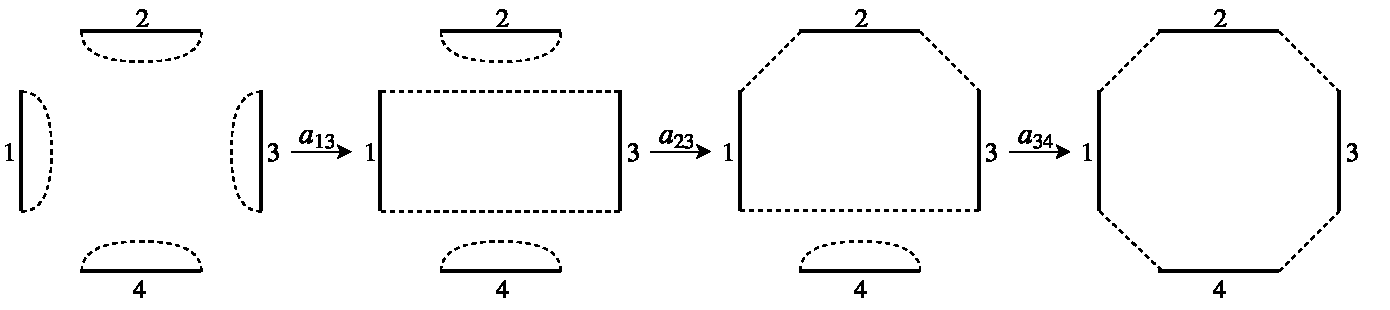
\includegraphics[width=\linewidth]{img/merge-into-cycle.pdf}
    \caption{Пример объеденения в цикл длины $4$}
    \label{merge-into-cycle}
\end{figure}

Отметим, что для наглядности, подписывая номера на блоках, мы имеем ввиду номера на соответствующих рёбрах.
Под соответствующим рёбром понимается ребро, наиболее близкое при движении по часовой стрелке.

Величина $a_{ij}$ на конкретном шаге могла получиться двумя способами: сначала выбран блок $i$, потом блок $j$, или же наоборот, $j$ потом $i$. Поэтому итоговую формулу будет необходимо домножить на $2^{m-1}$, так как всего шагов $m-1$.

Далее заметим, что для объединения в цикл не важен порядок операций, в котором они стоят. То есть сценарий $a_{13}, a_{23}, a_{34}$ равен сценарию $a_{23}, a_{13} a_{34}$ с точностью до перестановки. Следовательно, мы можем не учитывать конкретный порядок операций, а просто запоминать их множество, при этом домножив формулу на число перестановок, равное $(m-1)!$.

Полученный объект можно интерпретировать как множество рёбер в соответствующем остовном дереве. Пример подобного соответствия представлен на рис. ~\ref{tree-bijection}.
\begin{figure}[h!]
    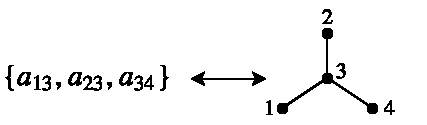
\includegraphics[width=3in]{img/tree-bijection.pdf}
    \caption{Пример биекции с остовными деревьями}
    \label{tree-bijection}
\end{figure}

Как известно, остовные деревья в графе размера $m$, кодируются кодами Прюфера \cite{prufer}, состоящими из $m-2$ чисел из множества ${1,2,\ldots,m}$. 
Нам необходимо получить сумму вероятностей по всем возможным сценариям слияния фиксированных блоков в цикл длины $m$, мы свели эту задачу к сумме по всем остовным деревьям размера $m$.
Степень вершины интерпретируется как число раз, когда соответствующее ребро было вовлечено в перестройку.
Теперь можно воспользоваться обобщенной формулой Кэли \cite{cayley}:
$$ \sum_T \prod_{i=0}^m p_i^{d_i(T)} 
= p_1 \ldots p_m (p_1 + \ldots + p_m) ^ {m - 2} \, . $$
С учётом возможных перестановок получим итоговую формулу:
$$2 ^ {m - 1} (m - 1)! p_1 \ldots p_m (p_1 + \ldots + p_m) ^ {m - 2} \, .$$

Важно отметить, что ввиду устройства операции ДРС, вероятности на рёбрах могут меняться.
Но для объединения в цикл нас интересует только сумма вероятностей в компоненте, а не отдельные $p_i$.
В процессе перераспределения сумма весов остаётся неизменной, а значит, наши рассуждения остаются верными.
\end{proof}

\subsection{Вычисление многомерного интеграла}
\begin{lemma}
$$
    \idotsint_{ \mathbb{R}^m_+} {
        \alpha_1 \cdot \ldots \cdot \alpha_m
        (\alpha_1 + \ldots + \alpha_m) ^ {m - 2}
        e ^ { -\sum_{i=1}^{m} ((\gamma + 1) \alpha_i)}
        \mathrm{d} \alpha_1 \ldots \mathrm{d} \alpha_m
    } = $$ $$ =  \frac
    {(3 m - 3)!}
    {(2 m - 1)! (\gamma + 1) ^ {3 m - 2}}
    \label{l-int}.
$$
\end{lemma}

\begin{proof}
Введём замену $t_i = \alpha_i (\gamma + 1)$:
$$
    \idotsint_{ \mathbb{R}^m_+} {
        \frac {t_1} {\gamma + 1} \cdot \ldots \cdot \frac {t_m} {\gamma + 1}
        \left(\frac {t_1 + \ldots + t_m} {\gamma + 1}\right) ^ {m - 2}
        e ^ { -\sum_{i=1}^{m} t_i}
        \frac {\mathrm{d} t_1} {\gamma + 1} \ldots \frac {\mathrm{d} t_m} {\gamma + 1}
    } = $$ $$ = \frac 1 {(\gamma + 1)^{3m-2}}
    \idotsint_{ \mathbb{R}^m_+} {
        t_1 \cdot \ldots \cdot t_m
        (t_1 + \ldots + t_m) ^ {m - 2}
        e ^ { -\sum_{i=1}^{m} t_i}
        \mathrm{d} t_1 \ldots \mathrm{d} t_m
    }
$$
Введём замену $u = t_1 + \ldots + t_m$:
$$
    \frac 1 {(\gamma + 1)^{3m-2}}
    \intop_{0}^{\infty}
    \idotsint_{ \sum_{i=1}^{m-1} t_i \leq u} {
        t_1 \ldots t_{n-1}
        \left(u - \sum_{i=1}^{m-1} t_i\right)
        u ^ {m - 2}
        e ^ {-u}
        \mathrm{d} t_1 \ldots \mathrm{d} t_{m-1} \mathrm{d} u
    } = $$ $$
    = \frac 1 {(\gamma + 1)^{3m-2}}
    \left(
        \intop_{0}^{\infty}
        \idotsint_{ \sum_{i=1}^{m-1} t_i \leq u} {
            t_1 \cdot \ldots \cdot t_{m-1}
            u ^ {m - 1}
            e ^ {-u}
            \mathrm{d} t_1 \ldots \mathrm{d} t_{m-1} \mathrm{d} u
        } -
        \right. $$ $$ \left. % hack for nice brackets
        - (m - 1)
        \intop_{0}^{\infty}
        \idotsint_{\sum_{i=1}^{m-1} t_i \leq u} {
            t_1^2 \cdot t_2 \cdot \ldots \cdot t_{m-1}
            u ^ {m - 2}
            e ^ {-u}
            \mathrm{d} t_1 \ldots \mathrm{d} t_{m-1} \mathrm{d} u
        }
    \right) = $$ $$
    = \frac 1 {(\gamma + 1)^{3m-2}}
    \left(
        \intop\nolimits_{0}^{\infty}
        \left(
            \idotsint_{ \sum_{i=1}^{m-1} t_i \leq u} {
                t_1 \cdot \ldots \cdot t_{m-1}
                \mathrm{d} t_1 \ldots \mathrm{d} t_{m-1}
            }
        \right)
        u ^ {m - 1}
        e ^ {-u}
        \mathrm{d} u
        \right. $$ $$ \left. % hack for nice brackets
        - (m - 1)
        \intop\nolimits_{0}^{\infty}
        \left(
            \idotsint_{ \sum_{i=1}^{m-1} t_i \leq u} {
                t_1^2 \cdot t_2 \cdot \ldots \cdot t_{m-1}
                \mathrm{d} t_1 \ldots \mathrm{d} t_{m-1}
            }
        \right)
        u ^ {m - 2}
        e ^ {-u}
        \mathrm{d} u
    \right) =
$$
$$ = \textrm{[по лемме ~\ref{subint1} и лемме ~\ref{subint2}]} = $$
$$
    = \frac 1 {(\gamma + 1)^{3m-2}}
    \left(
        \intop\nolimits_{0}^{\infty}
        \frac {u ^ {3m - 3} e ^ {-u}} {(2m - 2)!}
        \mathrm{d} u
        - (m - 1)
        \intop\nolimits_{0}^{\infty}
        \frac {2 u ^ {3m - 3} e ^ {-u}} {(2m - 1)!}
        \mathrm{d} u
    \right)
    = $$ $$ =
    \frac 1 {(\gamma + 1)^{3m-2}}
    \left(
        \frac 1 {(2m - 2)!}
        - \frac {2 (m - 1)} {(2m - 1)!}
    \right)
    \intop\nolimits_{0}^{\infty} u ^ {3m - 3} e ^ {-u} \mathrm{d} u
    = $$ $$ =
    \frac 1 {(\gamma + 1)^{3m-2}}
    \left(
        \frac {2m - 1 - 2m + 2} {(2m - 1)!}
    \right)
    \Gamma(3m-2)
    =
    \frac
    {(3 m - 3)!}
    {(2 m - 1)! (\gamma + 1) ^ {3 m - 2}}
$$
\end{proof}

\begin{lemma}
$$
    \idotsint_{ \sum_{i=1}^{n} t_i \leq u} {
        t_1 \cdot \ldots \cdot t_{n}
        \mathrm{d} t_1 \ldots \mathrm{d} t_{n}
    } =
    \frac {u ^ {2n}} {(2n)!}
    \label{subint1}.
$$
\end{lemma}
\begin{proof}
Доказательство проведём по индукции. База индукции, $n = 1$:
$$
    \intop_0^u {t \mathrm{d} t} =
    \frac {u ^ 2} 2 - \frac {0 ^ 2} 2 =
    \frac {u ^ 2} 2
$$
Шаг индукции, пусть выполняется:
$$
    \idotsint_{ \sum_{i=1}^{n} t_i \leq u} {
        t_1 \cdot \ldots \cdot t_{n}
        \mathrm{d} t_1 \ldots \mathrm{d} t_{n}
    } =
    \frac {u ^ {2n}} {(2n)!} \, .%точка
$$
Вычислим:
$$
    \idotsint_{ \sum_{i=1}^{n+1} t_i \leq u} {
        t_1 \cdot \ldots \cdot t_{n+1}
        \mathrm{d} t_1 \ldots \mathrm{d} t_{n+1}
    } =
    \intop_{0}^{u}
    \frac {(u - t_{n+1})^{2n}} {(2n)!} t_{n+1}
    \mathrm{d} t_{n+1}
    = $$ $$ =
    - \frac 1 {(2n)!}
    \intop_{0}^{u}
    t_{n+1} \mathrm{d} \left(\frac {(u - t_{n+1})^{2n + 1}} {2n + 1}\right)
    = $$ $$ =
    - \frac 1 {(2n)!}
    \left( \left.
        \frac {(u - t_{n+1})^{2n + 1} t_{n+1}} {2n + 1} \right|_0^u
        - \intop_{0}^{u}
        \frac {(u - t_{n+1}) ^ {2n+1}} {2n+1}
        \mathrm{d} t_{n+1}
    \right)
    = $$ $$ =
    \frac 1 {(2n + 1)!}
    \intop_{0}^{u}
    (u - t_{n+1}) ^ {2n+1}
    \mathrm{d} t_{n+1}
    =
    \frac 1 {(2n + 1)!}
    \left( \left.
        - \frac
        {(u - t_{n+1}) ^ {2n+2}}
        {2n + 2}
        \right|_0^u
    \right)
    = $$ $$ =
    \frac {u ^ {2n+2}} {(2n + 2)!}
$$
\end{proof}

\begin{lemma}
$$
    \idotsint_{ \sum_{i=1}^{n} t_i \leq u} {
        t_1^2 \cdot t_2 \cdot \ldots \cdot t_{n}
        \mathrm{d} t_1 \ldots \mathrm{d} t_{n}
    } =
    \frac {2 u ^ {2n + 1}} {(2n + 1)!}
    \label{subint2}.
$$
\end{lemma}
\begin{proof}
Доказательство проведём по индукции. База индукции, $n = 1$:
$$
    \intop_0^u {t^2 \mathrm{d} t} =
    \frac {u ^ 3} 3 - \frac {0 ^ 3} 3 =
    \frac {u ^ 3} 3
$$
Шаг индукции, пусть выполняется:
$$
    \idotsint_{ \sum_{i=1}^{n} t_i \leq u} {
        t_1^2 \cdot t_2 \cdot \ldots \cdot t_{n}
        \mathrm{d} t_1 \ldots \mathrm{d} t_{n}
    } =
    \frac {2 u ^ {2n + 1}} {(2n + 1)!}
$$
Вычислим:
$$
    \idotsint_{ \sum_{i=1}^{n+1} t_i \leq u} {
        t_1 \cdot t_2 \cdot \ldots \cdot t_{n+1}
        \mathrm{d} t_1 \ldots \mathrm{d} t_{n+1}
    } =
    \intop_{0}^{u}
    \frac {2 (u - t_{n+1})^{2n + 1}} {(2n + 1)!} t_{n+1}
    \mathrm{d} t_{n+1}
    =
$$ $$
    = - \frac 2 {(2n + 1)!}
    \intop_{0}^{u}
    t_{n+1} \mathrm{d} \left(
        \frac {(u - t_{n+1})^{2n + 2}} {2n + 2}
    \right)
    =
$$ $$
    =
    - \frac 2 {(2n + 1)!}
    \left( \left.
        \frac {(u - t_{n+1})^{2n + 2} t_{n+1}} {2n + 2} \right|_0^u
        - \intop_{0}^{u}
        \frac {(u - t_{n+1}) ^ {2n+2}} {2n+2}
        \mathrm{d} t_{n+1}
    \right)
    = $$ $$ =
    \frac 2 {(2n + 2)!}
    \intop_{0}^{u}
    (u - t_{n+1}) ^ {2n+2}
    \mathrm{d} t_{n+1}
    =
    \frac 2 {(2n + 2)!}
    \left( \left.
        - \frac
        {(u - t_{n+1}) ^ {2n+3}}
        {2n + 3}
        \right|_0^u
    \right)
    = $$ $$ =
    \frac {2 u ^ {2n+3}} {(2n + 3)!} \, .%точка
$$
\end{proof}


\section{Построение метода оценки истинного эволюционного расстояния}
Для оценки истинного эволюционного расстояния будем использовать кумулятивные статистики.
Первая статистика $\frac b n$ --- это нормированное число нетривиальных циклов:
$$\frac b n = 1 - \frac {c_1} n = 1 - \frac 1 {1 + \gamma} = \frac \gamma {1 + \gamma} \, .%точка 
$$

Вторая статистика $\frac d n$ --- это нормированнное минимальное эволюционное расстояние.
$$\frac d n = \sum_{m=2}^{\infty} \frac {c_m} n (m-1) =
1 - \frac
{(1 + \gamma)^2 ({}_2F_1\left(-\frac 2 3, -\frac 1 3, \frac 1 2, \frac {27 \gamma} {4 (1 + \gamma)^3}\right) - 1)}
{3 \gamma} \, .%точка
$$

Чтобы оценить истинное эволюционное расстояние, узнаем реальные $d$ и $b$ на текущем геноме.
Так как функция $\frac d b$ непрерывна и монотонна, мы можем найти её корень простым двоичным поиском, тем самым, мы узнаём $\gamma$.
Далее, зная $\gamma$, находим значение $\frac b n$.
Для того, чтобы предсказать $n$, достаточно разделить $b$ на $\frac b n$.
Всё что осталось --- вспомнить, что $k = \frac {\gamma n} 2$.

В листинге ~\ref{lst} приведен код данного метода на языке \textit{Python 3}:
\begin{algorithm}[!h]
\caption{Алгоритм оценки истинного эволючионного расстояния}
\label{lst}
\begin{lstlisting}[language=Python]
def predict_k(d, b):
    d_over_n = lambda x: 1 - (1 + x) ** 2 * (hyp2f1(-2 / 3, -1 / 3, 1 / 2, 27 * x / (4 * (1 + x) ** 3)) - 1) / (3 * x)
    b_over_n = lambda x: x / (1 + x)
    d_over_b = lambda r: lambda x: d_over_n(x) / b_over_n(x) - r

    gamma = optimize.bisect(d_over_b(d / b), 1e-6, 3, xtol=1e-4)
    b_n = b_over_n(gamma)
    n = b / b_n
    return n * gamma / 2
\end{lstlisting}
\end{algorithm}

Далее, проведём симуляции геномных перестроек на языке \textrm{Python} и оценим работу алгоритма для $\gamma \in [0,5, 2.0)$. Граница парсимонии находится на $\gamma = 0,5$, поэтому меньшие значения нас не интересуют. $\gamma \geq 2$ не рассматриваются, так как настолько удаленные геномы очень редки.

Для оценки работы алгоритма построен график распределения относительной ошибки $\frac {k_e - k} k$ от $\gamma$ вида <<ящик с усами>>. <<Ящикам>> соответсвуют $50 \, \%$ результатов, <<усам>> соответствуют $90 \, \%$. График приведен на рис. ~\ref{dir_est_05_20}. Как мы видим, $50 \, \%$ результатов оценки ошибаются не более, чем на $6 \, \%$, а $90 \, \%$ результатов ошибаются не более, чем на $10 \, \%$. Что является хорошим показателем для оценки в рамках модели.
\begin{figure}[h!]
    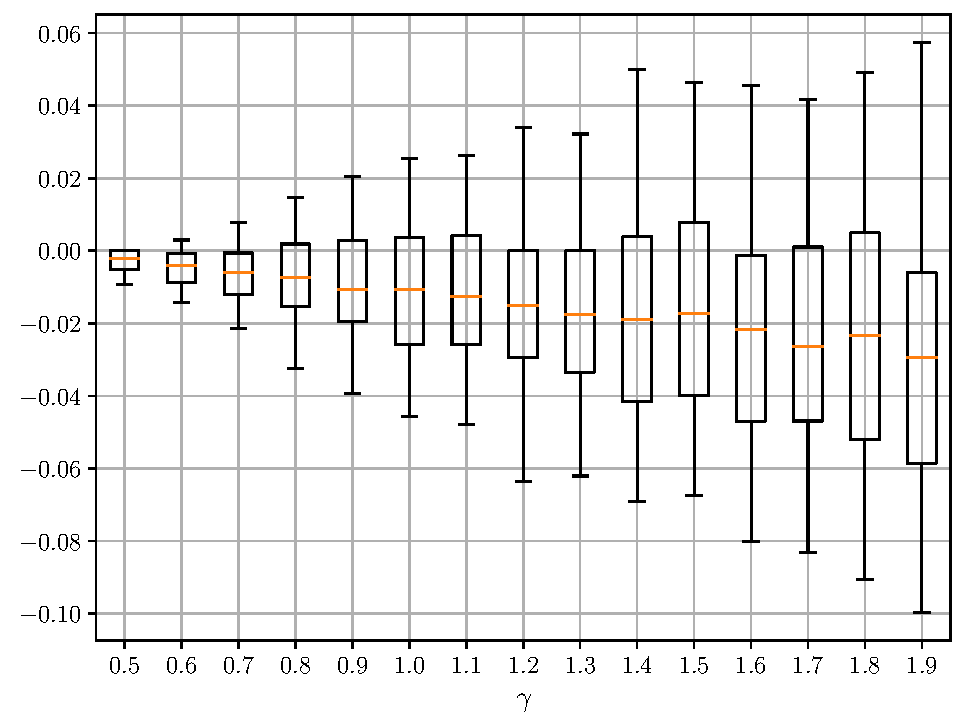
\includegraphics[width=0.8\linewidth]{img/dir_est_05_20.pdf}
    \caption{Зависимость распределения относительной ошибки $\frac {k_e - k} k$ от $\gamma$ в новом методе оценки}
    \label{dir_est_05_20}
\end{figure}

Также, в таблице ~\ref{tab-est-error} приведено соответствие среднего модуля ошибки $\frac {k_e - k} k$ в процентах от $\gamma \in [0,5, 2.0)$.

\begin{table}[!h]
  \caption{Средний модуль ошибки в процентах в зависимости от $\gamma$}\label{tab1}
  \centering
  \begin{tabular}{|*{4}{c|}}\hline
  \( \gamma \) & Средний модуль ошибки & \( \gamma \) & Средний модуль ошибки \\\hline
  $0.5$ & $0.3 \, \%$ & $1.3$ & $2.78 \, \%$ \\\hline
  $0.6$ & $0.58 \, \%$ & $1.4$ & $3.12 \, \%$ \\\hline
  $0.7$ & $0.86 \, \%$ & $1.5$ & $3.14 \, \%$ \\\hline
  $0.8$ & $1.24 \, \%$ & $1.6$ & $3.57 \, \%$ \\\hline
  $0.9$ & $1.59 \, \%$ & $1.7$ & $3.76 \, \%$ \\\hline
  $1.0$ & $1.88 \, \%$ & $1.8$ & $4.02 \, \%$ \\\hline
  $1.1$ & $2.1 \, \%$ & $1.9$ & $4.49 \, \%$ \\\hline
  $1.2$ & $2.43 \, \%$ & $2.0$ & $4.87 \, \%$ \\\hline
  \end{tabular}
  \label{tab-est-error}
\end{table}
%!!! я проглядел этот момент -- обычно смотрят на средний квадрат  ошибки, а не модуль. Но сейчас уже не меняйте

Как видно из рис. ~\ref{dir_est_05_20}, в данном методе оценки присутствует систематическая ошибка (предсказанное $k$ в среднем оказывается меньше, чем реальное).
Это связано с тем, что асимптотические оценки учитывают только компоненты первого порядка.
Но цикл заданной длины иногда может получаться ввиду распада цикла большей длины.

Для того, чтобы учесть этот факт, эмпирически оценим данную погрешность и учтём её.
Для $\gamma < 0.5$ погрешность для $\frac{d}{n}$ равняется $0$, а для $\gamma \geq 0.5$ она составляет $\frac{0.1}{\sqrt{n}}$.
Результаты работы метода оценки, учитывающего данную погрешность приведены на рис. ~\ref{dir_est_05_20_buffed}.
\begin{figure}[h!]
    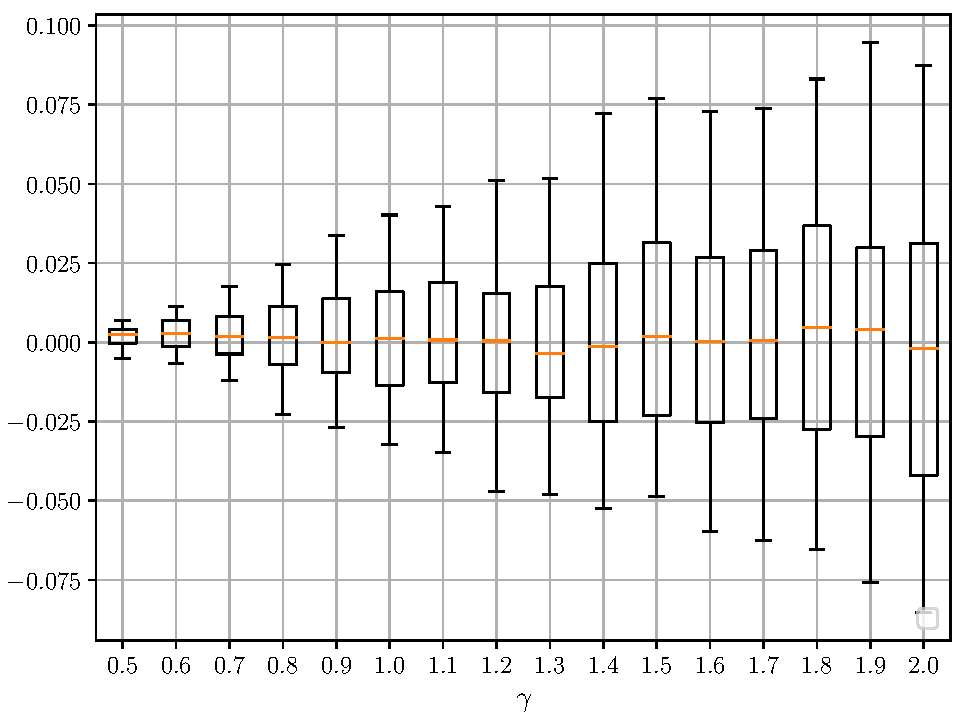
\includegraphics[width=0.8\linewidth]{img/dir_est_05_20_buffed.pdf}
    \caption{Зависимость распределения относительной ошибки $\frac {k_e - k} k$ от $\gamma$ в новом методе оценки с учетом эмпирической оценки на погрешность}
    \label{dir_est_05_20_buffed}
\end{figure}

\chapterconclusion
В главе 2 проведён теоретический анализ модели Дирихле и произведена асимптотическая оценка всех необходимых компонент, построены комбинаторные формулы для среднего числа компонент в общем случае. 

Предложен новый метод оценки истинного эволюционного расстояния в рамках этой модели, а также описана его реализация. Проведена оценка точности работы метода для $\gamma \in [0,5, 2.0)$.
\chapter{Сравнение}

\section{Сравнение эмпирических и аналитических результатов}
Для того, чтобы убедиться в правильности построения и анализа модели, проведём сравнение результатов, полученных эмпирическим и теоретическим способами.
Для этого произведем симуляцию на языке Python 3 и сравним полученные результаты с результатами теоретическими.
Помимо самого языка, для симуляции поведения модели использовалась библиотека для работы с графами networkx.
В данном случае использовано $200$ симулированных процессов.

\begin{figure}[h!]
    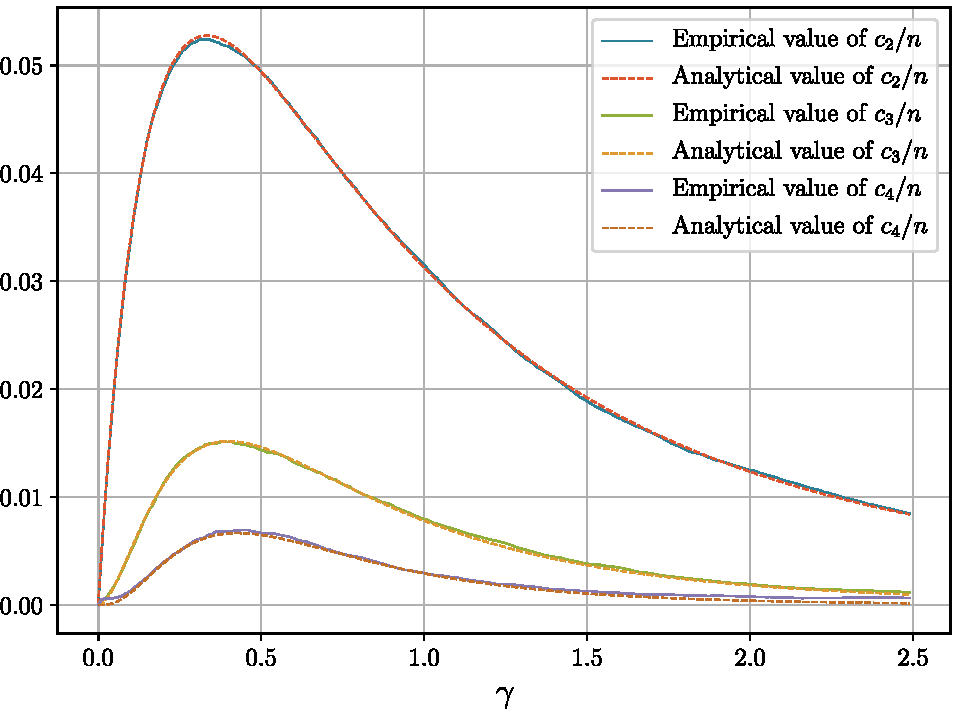
\includegraphics[width=0.9\linewidth]{img/cms_1.pdf}
    \caption{Сравнение эмпирических и теоретических результатов для нормированного количества циклов заданной длины}
    \label{cms}
\end{figure}

На рис.~\ref{cms} приведено сравнение результатов полученных эмпирическим и теоретическим способом.
Как мы видим, результаты достаточно хорошо совпадают и могут только незначительно отличаться при $\gamma \geq 1.5$, что связано с тем, что циклы меньшей длины могут получаться в результате распадения циклов большей длины.

Так как метод оценки основывается на статистиках $\frac b n$ и $\frac d n$ и их частном  $\frac b b$, построим подобный график и для них (рис.~\ref{d-b-n}).
\begin{figure}[h!]
    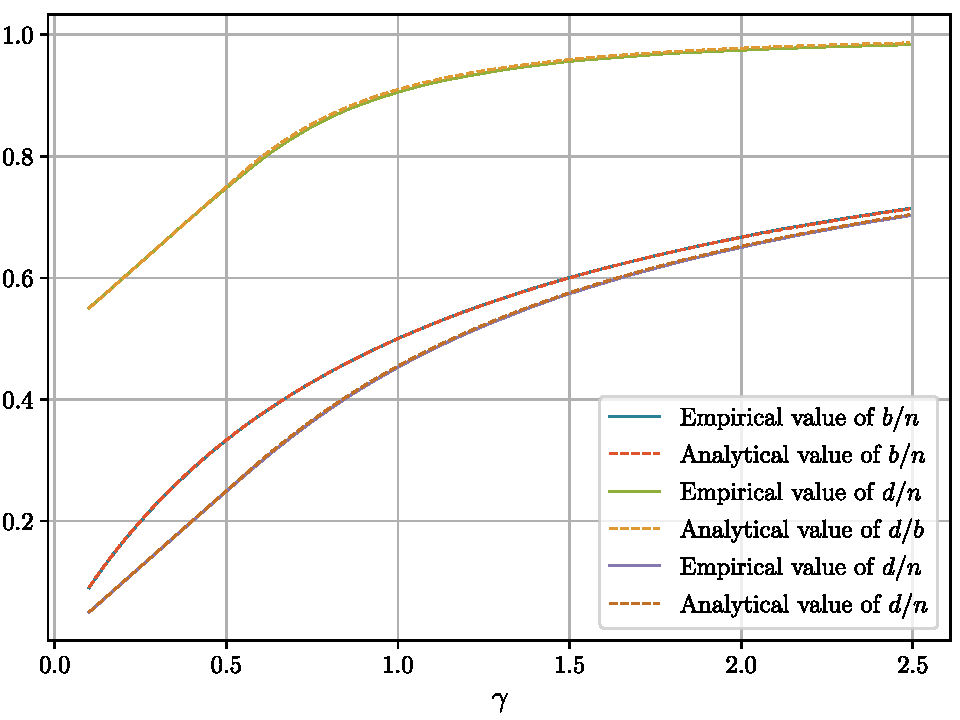
\includegraphics[width=0.9\linewidth]{img/d-b-n_1.pdf}
    \caption{Сравнение эмпирических и теоретических результатов для нормированного количества циклов заданной длины}
    \label{d-b-n}
\end{figure}
Как мы видим, в данном случае результаты совпадают ещё больше, и в некоторых моментах графики даже неразличимы.

\section{Сравнение с методом оценки Танье}
Для сравнения методов также будем использовать симулированные данные.
Для каждого $\gamma$ из отрезка $[0.3, 1)$ кратного $0.1$, попробуем предсказать, какое число шагов было сделано, и запишем соответствующую ошибку как $\frac {(k_e - k)} k$, где $k_e$ --- предсказанное число шагов, а $k$ --- реальное число шагов.
Для каждого соответствующего $\gamma$ было проведено 200 симуляций и построены соответствующие графики вида <<ящик с усами>>.
Как и ранее, <<ящик>> соответствует $50 \, \%$ результатов, а <<усы>>, в свою очередь, $90 \, \%$.

Важно отметить, что метод оценки не располагает информацией ни о реальном числе шагов, ни о количестве тривиальных циклов.
Вся информация, известная методу --- это количество циклов длин $l \geq 2$.

\begin{figure}[htb]
\centering
  \renewcommand{\thesubfigure}{а}
  \subfloat[Метод \textbf{Танье} на \textbf{больших} геномах]{%
    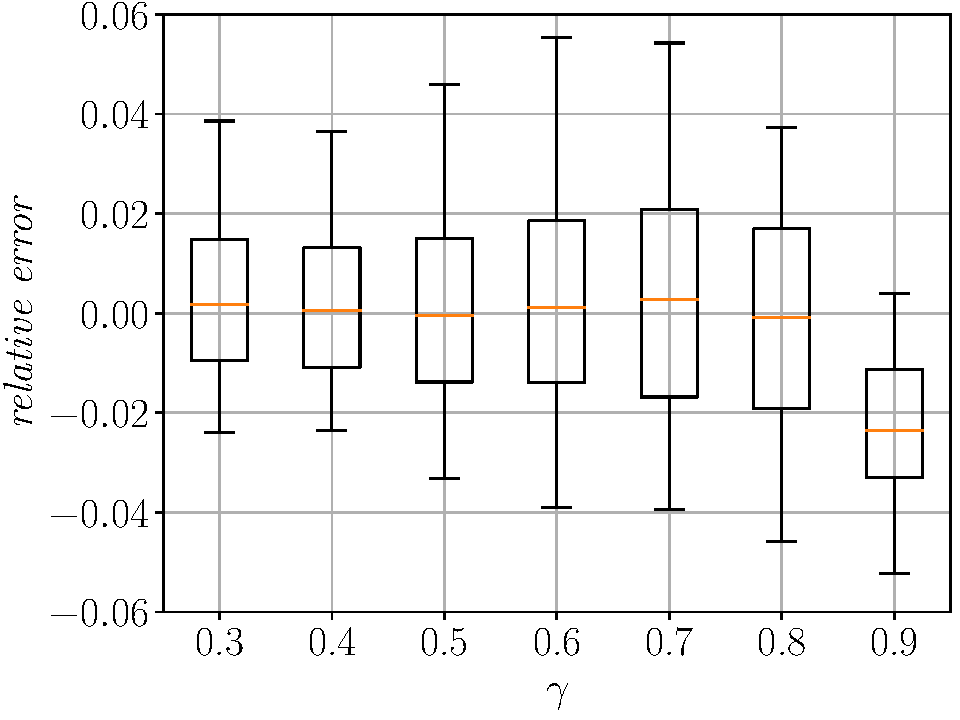
\includegraphics[width=.49\linewidth]{img/tan-est.pdf}}\hfill
  \renewcommand{\thesubfigure}{б}
  \subfloat[Метод \textbf{Танье} на \textbf{малых} геномах]{%
    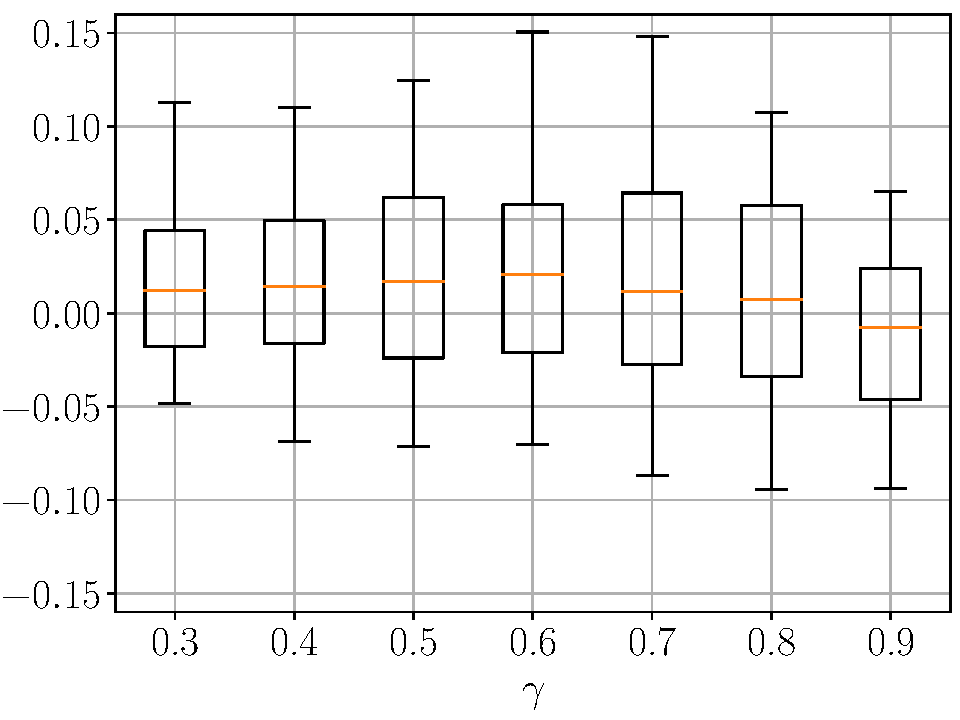
\includegraphics[width=.49\linewidth]{img/tan-est-small-n.pdf}} \\
  \renewcommand{\thesubfigure}{в}
  \subfloat[\textbf{Наш} метод  на \textbf{больших} геномах]{%
    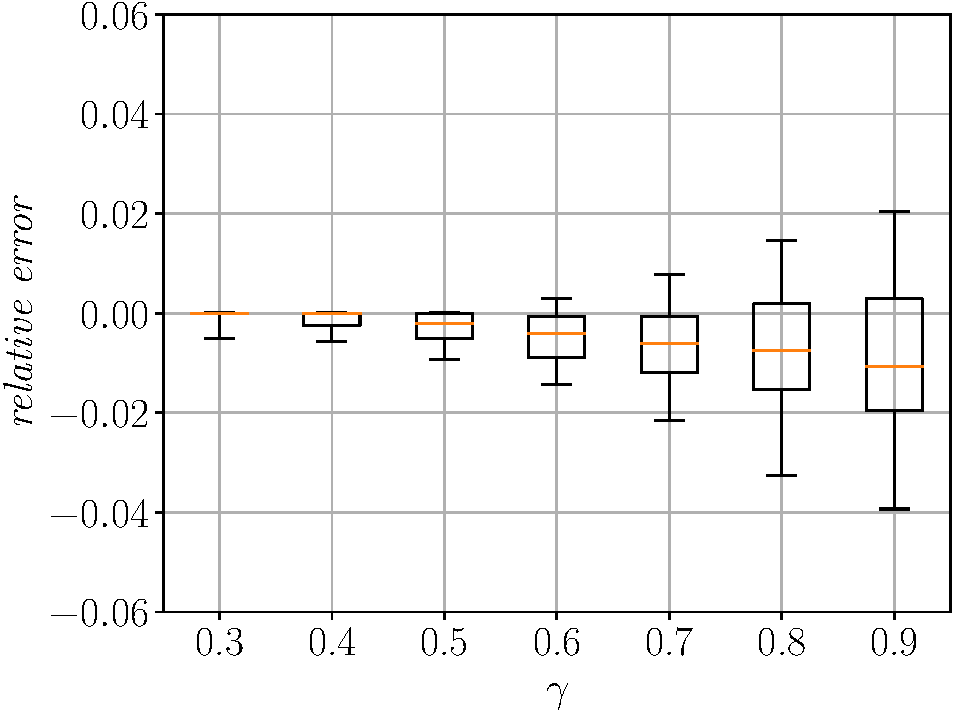
\includegraphics[width=.49\linewidth]{img/my-est.pdf}} \hfill
  \renewcommand{\thesubfigure}{г}
  \subfloat[\textbf{Наш} метод на \textbf{малых} геномах]{%
    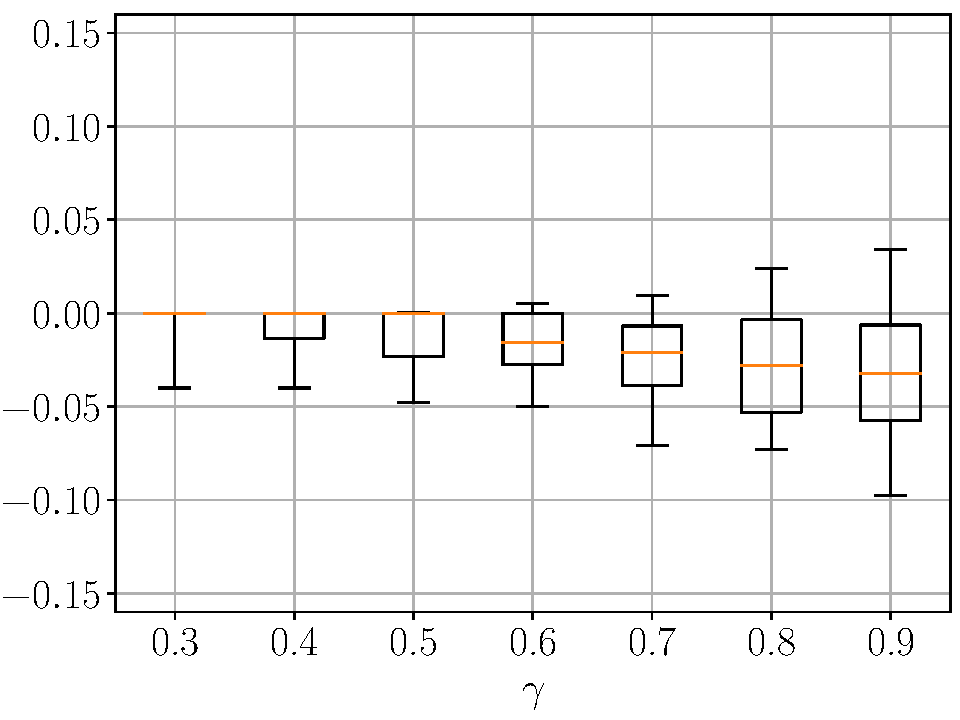
\includegraphics[width=.49\linewidth]{img/my-est-small-n.pdf}}
  \caption{Сравнение зависимости распределения относительной ошибки $\frac {k_e - k} k$ от $\gamma$ при оценке разными методами}
  \label{compare-methods}
\end{figure}


На рис.~\ref{compare-methods} показаны результаты работы разных методов для геномов разных размеров.
Для больших геномов $n$ находится в промежутке $[1000, 3000]$, для малых --- в промежутке $[200, 400]$.

Как мы видим, ошибка метода Танье для больших геномов находится в пределах $4 \, \%$ в $50 \, \%$ случаев, погрешность нашего же метода находится в пределах $2 \%$.
А в $90 \, \%$ случаев ошибка метода Танье находится в пределах $6 \, \%$, наш же метод ошибается не более, чем на $4 \, \%$.

Несмотря на то, что в нашей работе мы переходим к пределу по $n$, новый метод показывает лучшие результаты в сравнении с методом Танье.

Для малых геномов ошибка метода Танье находится в пределах $7 \, \%$ в $50 \, \%$ случаев, погрешность же нашего метода находится в пределах $6 \%$.
А в $90 \, \%$ случаев ошибка метода Танье находится в пределах $15 \, \%$, наш метод ошибается не более, чем на $10 \, \%$.

При больших $\gamma$ сравнить методы оценки не представляется возможным, так как метод Танье работает только при $k < \frac n 2$.

В главе 2 этой работы найдены теоретические оценки всех компонент, в то время как в работе \cite{fr-4} найдены оценки только для двух компонент, на которых построен метод оценивания. 
При этом одна из этих компонент $c_2$ имеет высокую дисперсию, что может негативно сказываться на точности оценки в случаях выбросов.

Оценки компонент, полученные в \cite{fr-4}, являются нелинейными, и для поиска оптимального решения используется решение системы двух нелинейных уравнений модифицированными градиентными методами.
Компонента $c_2$ немонотонна, что, однако, не влияет на результат.

В этой работе используются более простые и монотонные оценки, а для поиска корней - двоичный поиск.

Сравнение полученных оценок приведено в таблице ~\ref{comp-compare}:
\def\arraystretch{1.4}
\begin{table}[!h]
    \caption{Сравнение формул оценки необходимых компонент}
    \centering
    \begin{tabular}{|*{3}{c|}}\hline
            --              & Оценка Танье & Наша оценка \\\hline
            Оценка на $c_1$ &
            \(\displaystyle \sum_{l=0}^{\infty} \frac{(-2k)^l} {\prod_{u=0}^{l-1} (n+u)} \) &
            \(\displaystyle \frac {n^2} {2k + n} \) \\
        \hline
            Оценка на $c_2$ &
            \(\displaystyle k n^2 \sum_{l=0}^{\infty} \sum_{m=0}^{\infty} \frac{(-2(k-1))^{l+m}(l+1)(m+1)} {\prod_{u=0}^{l+m+1} (n+u)} \) &
            \(\displaystyle \frac {k n^4} {(2k + n)^4} \) \\
        \hline
    \end{tabular}
    \label{comp-compare}
\end{table}

Проведём сравнение реализаций данных методов.
Оба метода были реализованы на языке программирования \textit{Python 3}.
Так как метод Танье основывается на модифицированном градиентом спуске и имеет два нелинейных уравнения, была посчитана соответствующая матрица Якоби.
% тут можно написать формул для страху
Как было предложено в статье \cite{fr-4}, поиск оптимальных значений происходит с помощью метода \textit{optimize.root} из библиотеки \textit{scipy}.
Наш же метод использует метод двоичного поиска \textit{optimize.bisect} из той же библиотеки.

Измерения времени работы проведено на компьютере с процессором \textit{Core i5-5257U} и установленными \textit{Python} версии \textit{3.6.1} и библиотекой \textit{scipy} версии \textit{1.0.1}.

Важно отметить, что время работы ни одного из рассматриваемых методов оценки асимптотически никак не зависит от размера графа.
От размера графа зависит время, затрачиваемое на подсчёт необходимых компонент, и оно во всех случаях составляет $O(n)$, где $n$ --- число вершин в графе.
Подобная оценка достигается простым обходом в глубину.

Все измерения проводились на симулированных данных. Результаты приведены в таблице ~\ref{performance-compare}.
\begin{table}[!h]
    \caption{Сравнение работы методов}
    \centering
    \begin{tabular}{|*{3}{c|}}\hline
        -- & метод Танье & наш метод \\\hline
        \makecell{Среднее время работы \\ на малых геномах}       & 2.98 сек. & 0.00016 сек. \\\hline
        \makecell{Средний модуль ошибки \\ на малых геномах}      & 4.8 \%    & 2.1 \% \\\hline
        \makecell{Среднее время работы \\ на больших геномах}     & 3.02 сек. & 0.00017 сек. \\\hline
        \makecell{Средний модуль ошибки \\ на больших геномах}    & 1.99 \%   & 0.68 \% \\\hline
        Работает при $k \geq \frac n 2$                           & Нет       & Да \\\hline
        Реализация     & \makecell{Система уравнений и \\ модифицированный \\ градиентный спуск} & \makecell{Вещественный \\ двоичный поиск} \\\hline
    \end{tabular}
    \label{performance-compare}
\end{table}

\section{Применение метода к реальным данным}
\subsection{Семейство \emph{Rasacae}}

Для рассмотрения возьмем следующие геномы  видов из семейства \emph{Rosaceae}: \emph{Prunus} (слива), \emph{Fragaria} (клубника), \emph{Malus} (яблоко).
Геномные данные взяты из статьи \cite{real-data}.
Рассмотрим всевозможные пары этих геномов и запишем результаты в таблицу ~\ref{real-data-rasacae}.
\begin{table}[!h]
    \caption{Сравнения методов на реальных данных из семейства \emph{Rasacae}}
    \centering
    \begin{tabular}{|*{5}{c|}}\hline
        Пара геномов &  \makecell{Минимальное \\ расстояние}
                     & Наш метод
                     & Танье
                     & \makecell{Равновероятная \\ модель} \\\hline
        \emph{Prunus} --- \emph{Fragaria}    & 273 & 297 & 284 & 283     \\\hline
        \emph{Prunus} --- \emph{Malus}     & 261 & 263 & 258 & 261    \\\hline
        \emph{Fragaria} --- \emph{Malus} & 414 & 461 & 426 & 435   \\\hline
    \end{tabular}
    \label{real-data-rasacae}
\end{table}

Как можно увидеть из таблицы, истинное эволюционное растояние в рамках нашей модели может отличаться от минимального на $11 \, \%$ (это достигается в паре <<\emph{Prunus} --- \emph{Fragaria}>>).
В то время как классический подход (равновероятная модель) к оценке истинного расстояния показывает разницы всего в $5 \, \%$.
Заметим, что разница такого порядка является статистически значимой; вероятность того, что она  является результатом погрешности измерений не превосходит $1 \, \%$.

Аналогичная ситуация происходит на паре <<\emph{Prunus} --- \emph{Fragaria}>>, в рамках нашей модели разница с минимальным расстоянием достигает $8.7 \, \%$, а в рамках равновероятной модели эта цифра составляет $4 \, \%$.

Пара <<\emph{Prunus} --- \emph{Malus}>> в нашей модели находится немного за границей парсимонии, а в рамках модели равновероятной перед ней.
Поэтому различие в минимальном и истинном расстоянии мы видим только в рамках нашей модели.

Метод Танье на предложенных данных показывает себя чуть хуже.
Результаты его работы примерно равны результатам оценщика классического.
За исключением того факта, что в паре <<\emph{Prunus} --- \emph{Malus}>> он показал результат меньший, чем минимальное расстояние.
Вероятно это связно с тем, что произошёл выброс по компоненте $c_2$.

\subsection{Класс \emph{Mammalian}}
Для следующего рассмотрения возьмем геномы  видов из класса \emph{Mammalian} (млекопитающие): \emph{Rat} (крыса), \emph{Chimpanzee} (шимпанзе), \emph{Dog} (собака), \emph{Mouse} (мышь), \emph{Macaque} (макака), \emph{Human} (человек).
Рассмотрим всевозможные пары этих геномов и запишем результаты в таблицу ~\ref{real-data-mammalian}.
\begin{table}[!h]
    \caption{Сравнения методов на реальных данных из класса \emph{Mammalian}}
    \centering
    \begin{tabular}{|*{5}{c|}}\hline
        Пара геномов &  \makecell{Минимальное \\ расстояние}
                     & Наш метод
                     & Танье
                     & \makecell{Равновер. \\ модель} \\\hline
                    \emph{Chimpanzee} --- \emph{Dog}    & 312 & 312 & 287 & 312     \\\hline
                    \emph{Chimpanzee} --- \emph{Human}    & 22 & 22 & 22 & 22     \\\hline
                    \emph{Chimpanzee} --- \emph{Mouse}    & 420 & 426 & 379 & 420     \\\hline
                    \emph{Chimpanzee} --- \emph{Macaque}    & 115 & 115 & 118 & 115     \\\hline
                    \emph{Chimpanzee} --- \emph{Rat}    & 724 & 724 & 703 & 724     \\\hline
                    \emph{Dog} --- \emph{Human}    & 304 & 304 & 278 & 304     \\\hline
                    \emph{Dog} --- \emph{Mouse}    & 450 & 456 & 409 & 450     \\\hline
                    \emph{Dog} --- \emph{Macaque}    & 301 & 301 & 275 & 301     \\\hline
                    \emph{Dog} --- \emph{Rat}    & 756 & 756 & 733 & 756     \\\hline
                    \emph{Human} --- \emph{Mouse}    & 408 & 414 & 370 & 408     \\\hline
                    \emph{Human} --- \emph{Macaque}    & 106 & 106 & 109 & 106     \\\hline
                    \emph{Human} --- \emph{Rat}    & 714 & 714 & 694 & 714     \\\hline
                    \emph{Mouse} --- \emph{Macaque}    & 407 & 407 & 367 & 407     \\\hline
                    \emph{Mouse} --- \emph{Rat}    & 454 & 454 & 464 & 454     \\\hline
                    \emph{Macaque} --- \emph{Rat}    & 706 & 706 & 690 & 706     \\\hline
    \end{tabular}
    \label{real-data-mammalian}
\end{table}

Как можно увидеть из таблицы, в рамках модели с равновероятными поломками рёбер, все пары геномов находятся на стадии парсимонии. 
То есть оценка на истинное эволюционное расстояние совпадает с минимальным расстоянием.

В рамках нашей модели три пары геномов находятся за границей парсимонии и отличаются примерно на $1.5 \, \%$. 
Этими парами являются: \emph{Chimpanzee} --- \emph{Mouse}, \emph{Dog} --- \emph{Mouse} и \emph{Human} --- \emph{Mouse}.
Это говорит о том, что \emph{Mouse} более удалена от остальных видов из класса \emph{Mammalian} (млекопитающие) взятого набора.

Метод Танье на рассматриваемых видах показывает себя неудовлетворительно.
В $11$ парах из $15$ (\emph{Chimpanzee} --- \emph{Dog}, \emph{Chimpanzee} --- \emph{Mouse}, \emph{Chimpanzee} --- \emph{Rat}, \emph{Dog} --- \emph{Human}, \emph{Dog} --- \emph{Mouse}, \emph{Dog} --- \emph{Macaque}, \emph{Dog} --- \emph{Rat}, \emph{Human} --- \emph{Mouse}, \emph{Human} --- \emph{Rat}, \emph{Mouse} --- \emph{Macaque}, \emph{Macaque} --- \emph{Rat}) оценка на истинное расстояние меньше, чем минимальное расстояние. 
Причём, подобная ошибка достигает $9.8 \, \%$ в случае пары \emph{Mouse} --- \emph{Macaque} и некоторых других, что показывает неприменимость метода Танье к данным видам. 
Данная ошибка, вероятнее всего, связана с выбросом по компоненте $c_2$.

\subsection{Род \emph{Shigella}}
Для последнего рассмотрения возьмем геномы  видов из класса \emph{Shigella}: \emph{Shigella sonnei Ss046}, \emph{Shigella boydii Sb227}, \emph{Shigella boydii CDC 3083 94}, \emph{Shigella flexneri 2a}, \emph{Shigella flexneri 5 8401}, \emph{Shigella flexneri 2a 2457T}.
Рассмотрим всевозможные пары этих геномов и запишем результаты в таблицу ~\ref{real-data-shigella}.
\begin{table}[!h]
    \caption{Сравнения методов на реальных данных из рода \emph{Shigella}}
    \centering
    \begin{tabular}{|*{5}{c|}}\hline
        Пара геномов &  \makecell{Мин. \\ расст.}
                     & Наш метод
                     & Танье
                     & \makecell{Равновер. \\ модель} \\\hline
                    \makecell{ \emph{S. s. Ss046} --- \emph{S. b. Sb227} }    & 32 & 32 & 31 & 32     \\\hline
                    \makecell{ \emph{S. s. Ss046} --- \emph{S. b. CDC 3083 94} }    & 44 & 46 & 47 & 44     \\\hline
                    \makecell{ \emph{S. s. Ss046} --- \emph{S. f. 2a} }    & 43 & 45 & 46 & 43     \\\hline
                    \makecell{ \emph{S. s. Ss046} --- \emph{S. f. 5 8401} }    & 40 & 40 & 40 & 40     \\\hline
                    \makecell{ \emph{S. s. Ss046} --- \emph{S.f. 2a 2457T} }    & 35 & 35 & 40 & 35     \\\hline
                    \makecell{ \emph{S. b. Sb227} --- \emph{S. b. CDC 3083 94} }    & 42 & 42 & 45 & 42     \\\hline
                    \makecell{ \emph{S. b. Sb227} --- \emph{S. f. 2a} }    & 45 & 45 & 46 & 45     \\\hline
                    \makecell{ \emph{S. b. Sb227} --- \emph{S. f. 5 8401} }    & 40 & 40 & 40 & 40     \\\hline
                    \makecell{ \emph{S. b. Sb227} --- \emph{S.f. 2a 2457T} }    & 35 & 35 & 34 & 35     \\\hline
                    \makecell{ \emph{S. b. CDC 3083 94} --- \emph{S. f. 2a} }    & 9 & 9 & 9 & 9     \\\hline
                    \makecell{ \emph{S. b. CDC 3083 94} --- \emph{S. f. 5 8401} }    & 14 & 14 & 15 & 14     \\\hline
                    \makecell{ \emph{S. b. CDC 3083 94} --- \emph{S.f. 2a 2457T} }    & 28 & 28 & 29 & 28     \\\hline
                    \makecell{ \emph{S. f. 2a} --- \emph{S. f. 5 8401} }    & 11 & 11 & 12 & 11     \\\hline
                    \makecell{ \emph{S. f. 2a} --- \emph{S.f. 2a 2457T} }    & 29 & 29 & 30 & 29     \\\hline
                    \makecell{ \emph{S. f. 5 8401} --- \emph{S.f. 2a 2457T} }    & 24 & 24 & 25 & 24     \\\hline
    \end{tabular}
    \label{real-data-shigella}
\end{table}

Как можно увидеть из таблицы для видов из рода \emph{Shigella}, в рамках модели с равновероятными поломками рёбер все пары геномов опять же находятся на стадии парсимонии. 
То есть минимальное расстояние совпадает с оценкой на истинное эволюционное расстояние.

При этом в рамках нашего метода $2$ пары (\emph{S. s. Ss046} --- \emph{S. b. CDC 3083 94}, \emph{S. s. Ss046} --- \emph{S. f. 2a}) выходят за границу парсимонии.
Оценка на расстояние отличается от минимального отличается всего на $2$ шага, но эти $2$ шага дают отличие на $4.5 \, \%$, что является заметным различием.

Метод Танье на видах рода \emph{Shigella} показывает себя лучше, чем на предыдущих.
Только в случае одной пары оценка на истинное расстояние оказывается меньше, чем  минимальное расстояние(\emph{S. b. Sb227} --- \emph{S.f. 2a 2457T}).
На тех же двух парах, которые выходили за границу парсимониив в нашем методе, также достигается выход за границу. 
Но выход за подобную границу достигается и на многих других парах:
\emph{S. s. Ss046} --- \emph{S.f. 2a 2457T},
\emph{S. b. Sb227} --- \emph{S. b. CDC 3083 94},
\emph{S. b. Sb227} --- \emph{S. f. 2a},
\emph{S. b. CDC 3083 94} --- \emph{S. f. 5 8401},
\emph{S. b. CDC 3083 94} --- \emph{S.f. 2a 2457T},
\emph{S. f. 2a} --- \emph{S. f. 5 8401},
\emph{S. f. 2a} --- \emph{S.f. 2a 2457T},
\emph{S. f. 5 8401} --- \emph{S.f. 2a 2457T}.

\subsection{Оценка производительности на реальных данных}
Несмотря на то, что скорость работы метода оценки не зависит асимптотически от размера генома, для полноты картины проведём оценку на скорость работы методов на реальных данных.
Для этого замерим среднее время работы каждого метода на всевозможных парах реальных данных рассмотренных выше, включая время на преобразование генома в граф точек и вычисление необходимых компонент. 
Результаты приведены в таблице ~\ref{real-data-time}.
\begin{table}[!h]
    \caption{Среднее время работы методов}
    \centering
    \begin{tabular}{|*{4}{c|}}\hline
        Набор геномов & Наш метод
                      & Танье
                      & \makecell{Равновероятная \\ модель} \\\hline
        Семейство \emph{Rasacae} & 0.012 сек. & 3.13 сек. & 0.015 сек. \\\hline
        Класс \emph{Mammalian}   & 0.027 сек. & 3.55 сек. & 0.037 сек. \\\hline
        Род \emph{Shigella}      & 0.004 сек. & 2.93 сек. & 0.008 сек. \\\hline
    \end{tabular}
    \label{real-data-time}
\end{table}

\chapterconclusion
В главе 3 был проведен эмпирический анализ модели и сравнение с теоретическими результатами.
Также было проведено сравнение нового метода оценки с методом, предложенным в \cite{fr-4}. Это сравнение показало более высокие точность, эффективность и применимость указанного метода.

Разные методы оценки расстояния были применены к реальным данным.
Основываясь на этих данных показано, что истинное эволюционное расстояние может отличаться от минимального до $11 \, \%$.
%!!! это Вы  как-то скромно, мы  же не все на свете пары организмов перебрали.
%!!! но оставьте так
И наконец, ввиду измененной границы парсимонии, показано, что в рамках рассматриваемой модели парсимония может не достигаться там, где она достигалась ранее.
\startconclusionpage

В рамках выпускной квалификационной работы был предложен новый метод оценки истинного эволюционного расстояния между геномами в рамках модели, предложенной в \cite{fr-4}.
Показана высокая точность данного метода.

Новый метод базируется на асимптотическом анализе комбинаторных формул для среднего числа компонент в общем случае.
Все формулы выведены в общем виде для любых весов $p_i$ на рёбрах, при этом существенно использовалась формула Кэли \cite{cayley}.
Для получения конечных результатов, вычисляется многомерный интеграл по плотности вероятности для стационарного распределения рассматриваемой модели.
При необходимости данные формулы могут быть применены и к другим распределениям весов на рёбрах.

В работе произведено сравнение эмпирических и теоретических результатов данной модели.
Показана их высокая согласованность.

Также выполнено сравнение нового метода оценки с методом, предложенным в \cite{fr-4}. 
Показано, что новый метод дает более высокие точность, применимость и эффективность.

Разные методы оценки эволюционного расстояния были применены к реальным  данным геномов из семейства \emph{Rosaceae}, класса \emph{Mammalian} и рода \emph{Shigella}.
Показано, что истинное эволюционное может существенно отличаться от минимального, уточнена граница парсимонии.
\printmainbibliography

\end{document}
